\chapter{Artificial Neural Networks and MLPs with Keras}

\newcommand{\lcTrainLoss}{\addplot[very thick,mlblue] coordinates {(1,0.7239) (2,0.4894) (3,0.4433) (4,0.4153) (5,0.395) (6,0.379) (7,0.3656) (8,0.3538) (9,0.3433) (10,0.3338) (11,0.325) (12,0.3168) (13,0.309) (14,0.3018) (15,0.2951) (16,0.2887) (17,0.2828) (18,0.277) (19,0.2715) (20,0.2664) (21,0.2613) (22,0.2565) (23,0.2516) (24,0.2471) (25,0.2425) (26,0.2382) (27,0.234) (28,0.2298) (29,0.2256) (30,0.2218)};}
\newcommand{\lcValLoss}{\addplot[very thick,mlorange,dashed] coordinates {(1,0.5026) (2,0.4473) (3,0.4232) (4,0.408) (5,0.3978) (6,0.3895) (7,0.3846) (8,0.378) (9,0.3733) (10,0.368) (11,0.3638) (12,0.3604) (13,0.3584) (14,0.3556) (15,0.3538) (16,0.3527) (17,0.3509) (18,0.3498) (19,0.3487) (20,0.3498) (21,0.3474) (22,0.3473) (23,0.3457) (24,0.3466) (25,0.3462) (26,0.3466) (27,0.346) (28,0.3464) (29,0.3462) (30,0.3454)};}
\newcommand{\lcTrainAcc}{\addplot[very thick,mlblue] coordinates {(1,0.7616) (2,0.83) (3,0.8448) (4,0.8548) (5,0.8605) (6,0.8667) (7,0.8712) (8,0.8747) (9,0.8783) (10,0.8815) (11,0.8845) (12,0.8871) (13,0.8895) (14,0.8923) (15,0.8941) (16,0.8964) (17,0.8986) (18,0.9008) (19,0.9029) (20,0.9046) (21,0.9057) (22,0.9084) (23,0.9101) (24,0.9117) (25,0.9137) (26,0.9157) (27,0.9175) (28,0.919) (29,0.9209) (30,0.9223)};}
\newcommand{\lcValAcc}{\addplot[very thick,mlorange,dashed] coordinates {(1,0.8298) (2,0.842) (3,0.8472) (4,0.8552) (5,0.858) (6,0.8602) (7,0.8592) (8,0.8628) (9,0.8664) (10,0.8686) (11,0.869) (12,0.872) (13,0.8724) (14,0.8726) (15,0.8736) (16,0.874) (17,0.8736) (18,0.8744) (19,0.8742) (20,0.875) (21,0.8758) (22,0.8768) (23,0.878) (24,0.8778) (25,0.8786) (26,0.8798) (27,0.8798) (28,0.8804) (29,0.8802) (30,0.8812)};}


\begin{objectives}
After studying this chapter you will be able to:
\begin{itemize}
  \item explain the \textbf{artificial neuron} and compare it with a biological neuron;
  \item train a \textbf{perceptron} by hand and explain why a single neuron cannot solve \textbf{XOR};
  \item describe the architecture of a \textbf{multilayer perceptron (MLP)}, count its parameters and compute a \textbf{forward pass} by hand;
  \item compare the common \textbf{activation functions} and explain why non-linearity is essential;
  \item explain \textbf{backpropagation} and carry it out by hand on a small network;
  \item choose the \textbf{output layer} and \textbf{loss function} for regression, binary and multi-class problems;
  \item build, train, evaluate and tune MLPs with \textbf{Keras} (Sequential and Functional API);
  \item control \textbf{overfitting} with dropout, L2 regularisation and early stopping;
  \item answer 2-, 5- and 10-mark university questions on neural networks.
\end{itemize}
\end{objectives}

\begin{pullquote}[--- Alan Turing, 1950]
We can only see a short distance ahead, but we can see plenty there that needs to be done.
\end{pullquote}

Unit~V is about \textbf{neural networks}, the models behind modern image recognition, speech assistants and language translation. A neural network is built from many very simple units, \textbf{neurons}. In this chapter we start with a single neuron, grow it into a network, understand how the network \emph{learns} (backpropagation) and then build real networks in Python with \textbf{Keras}.

%====================================================================
\section{From Biological to Artificial Neurons}

\subsection{The Biological Inspiration}

The human brain contains about 86 billion neurons. Each neuron receives electrical signals from other neurons through its \textbf{dendrites}, adds them up in the cell body (\textbf{soma}), and, if the total is strong enough, sends a pulse along its long \textbf{axon} to other neurons. Learning corresponds to changing the \emph{strength} of the connections.

\begin{definition}[: Artificial neuron]
An \textbf{artificial neuron} computes a weighted sum of its inputs plus a bias and passes the result through an \textbf{activation function} $\varphi$:
\[
  z=\sum_{i=1}^{n}w_ix_i+b=\vect w\cdot\vect x+b,\qquad a=\varphi(z).
\]
The \textbf{weights} $w_i$ say how important each input is (they play the role of connection strengths), the \textbf{bias} $b$ shifts the threshold at which the neuron fires, and $a$ is the \textbf{output} (activation).
\end{definition}

\begin{definition}[: Artificial neural network (ANN)]
An \textbf{artificial neural network} is a model made of many artificial neurons arranged in \textbf{layers} and connected by weights. The weights are learned from data by minimising a loss function with gradient descent.
\end{definition}

\begin{figure}[!htbp]
\centering
\resizebox{\linewidth}{!}{%
\begin{tikzpicture}
% ---------------- biological neuron ----------------
\node[font=\small\bfseries] at (2.6,3.6) {Biological neuron};
\fill[mlpurple!25,draw=mlpurple,thick] (2.6,1.3) circle (0.65);
\node[font=\scriptsize] at (2.6,1.3) {soma};
\foreach \a/\b in {0.4/2.8,0.6/1.3,0.4/-0.2,1.4/3.1,1.5/-0.6} {\draw[mlpurple,thick] (2.0,1.3)--(\a,\b);}
\draw[mlpurple,thick] (0.4,2.8)--(-0.2,3.1); \draw[mlpurple,thick] (0.4,2.8)--(0.0,2.4);
\draw[mlpurple,thick] (0.6,1.3)--(0.0,1.6); \draw[mlpurple,thick] (0.6,1.3)--(0.0,1.0);
\draw[mlpurple,thick] (0.4,-0.2)--(-0.2,0.1); \draw[mlpurple,thick] (0.4,-0.2)--(0.0,-0.5);
\node[font=\scriptsize,mlpurple,anchor=east] at (0.0,3.3) {dendrites};
\draw[mlpurple,very thick] (3.25,1.3)--(6.6,1.3);
\foreach \y in {1.8,1.3,0.8} {\draw[mlpurple,thick] (6.6,1.3)--(7.2,\y); \fill[mlpurple] (7.2,\y) circle (0.08);}
\node[font=\scriptsize,mlpurple,anchor=north] at (4.9,1.2) {axon};
\node[font=\scriptsize,mlpurple,anchor=south west] at (6.8,2.0) {to next neurons};
\node[font=\scriptsize,align=center] at (1.0,0.3) {inputs\\arrive here};
% ---------------- arrow ----------------
\draw[-{Stealth},ultra thick,gray] (8.1,1.3)--(9.0,1.3);
% ---------------- artificial neuron ----------------
\begin{scope}[xshift=9.6cm]
\node[font=\small\bfseries] at (3.5,3.6) {Artificial neuron};
\foreach \i/\y in {1/2.4,2/1.3,3/0.2} {
  \node[circle,draw=mlblue,fill=mlblue!12,thick,minimum size=0.7cm] (x\i) at (0,\y) {$x_\i$};
}
\node[circle,draw=mlorange,fill=mlorange!14,very thick,minimum size=1.3cm] (s) at (3.0,1.3) {$\Sigma+b$};
\node[draw=mlgreen,fill=mlgreen!14,thick,rounded corners,minimum height=0.9cm,minimum width=1.0cm] (f) at (5.0,1.3) {$\varphi$};
\node[circle,draw=mlred,fill=mlred!10,thick,minimum size=0.7cm] (y) at (6.8,1.3) {$a$};
\foreach \i in {1,2,3} \draw[-{Stealth},thick] (x\i)--(s);
\node[font=\scriptsize,fill=white,inner sep=1pt] at (1.5,2.1) {$w_1$};
\node[font=\scriptsize,fill=white,inner sep=1pt] at (1.5,1.3) {$w_2$};
\node[font=\scriptsize,fill=white,inner sep=1pt] at (1.5,0.5) {$w_3$};
\draw[-{Stealth},thick] (s)--(f); \draw[-{Stealth},thick] (f)--(y);
\node[font=\scriptsize,anchor=south] at (4.0,1.4) {$z$};
\end{scope}
\pic[scale=1.1] at (10.2,-1.0) {smile};
\bubble[text width=5.2cm]{14.4,-1.0}{10.7,-0.95}{I add up my weighted inputs, and if the total is big enough, I \textbf{fire}!}
\end{tikzpicture}}
\caption{A biological neuron and its mathematical model.}\label{fig:neuron}
\end{figure}

\begin{explain}
\textbf{Left:} a biological neuron. Signals enter through the \textbf{dendrites} (left), are combined in the \textbf{soma} (the body) and the result travels out along the \textbf{axon} to the next neurons. \textbf{Right:} the artificial copy. The inputs $x_1,x_2,x_3$ (blue) are multiplied by the weights $w_1,w_2,w_3$ (the strengths of the connections), added up together with the bias $b$ in the orange circle to give $z=\vect w\cdot\vect x+b$, and passed through the activation function $\varphi$ (green) to give the output $a=\varphi(z)$. This tiny calculation is repeated millions of times in a large network.
\end{explain}

\begin{center}
\begin{tabular}{@{}cp{11cm}@{}}
\toprule
\textbf{Year} & \textbf{Milestone}\\
\midrule
1943 & McCulloch and Pitts propose the first mathematical model of a neuron\\
1958 & Rosenblatt invents the \textbf{perceptron}\\
1969 & Minsky and Papert show that a single perceptron cannot learn XOR; interest in neural networks fades\\
1986 & Rumelhart, Hinton and Williams popularise \textbf{backpropagation} for training multilayer networks\\
2012 & A deep convolutional network wins the ImageNet competition; the \textbf{deep learning} boom begins\\
\bottomrule
\end{tabular}
\end{center}

\subsection{Logic with Neurons}

With the step activation $\varphi(z)=1$ if $z>0$ and $0$ otherwise, one neuron can implement simple logic gates:

\begin{center}
\begin{tabular}{@{}lccc@{}}
\toprule
\textbf{Gate} & \textbf{Weights} & \textbf{Bias} & \textbf{Output}\\
\midrule
AND & $(1,\ 1)$ & $-1.5$ & $\text{step}(x_1+x_2-1.5)$\\
OR & $(1,\ 1)$ & $-0.5$ & $\text{step}(x_1+x_2-0.5)$\\
NOT & $(-1)$ & $+0.5$ & $\text{step}(0.5-x_1)$\\
\bottomrule
\end{tabular}
\end{center}

For example, AND with inputs $(1,1)$: $z=1+1-1.5=0.5>0\Rightarrow1$; with $(1,0)$: $z=-0.5\Rightarrow0$. But a single neuron \textbf{cannot} compute the \textbf{XOR} (exclusive or) function, which is $1$ when the inputs \emph{differ}. In the plane, the points $(0,1)$ and $(1,0)$ (output $1$) lie on one diagonal and $(0,0)$ and $(1,1)$ (output $0$) on the other: no single straight line separates them.

\begin{figure}[!htbp]
\centering
\resizebox{\linewidth}{!}{%
\begin{tikzpicture}
% ---------------- XOR scatter ----------------
\node[font=\small\bfseries] at (2.0,4.4) {(a) XOR is not linearly separable};
\draw[gray!30] (-0.4,-0.4) grid (2.4,2.4) ;
\draw[-{Stealth},thick] (-0.4,0)--(2.6,0) node[right,font=\small]{$x_1$};
\draw[-{Stealth},thick] (0,-0.4)--(0,2.6) node[above,font=\small]{$x_2$};
\foreach \x/\y in {0/0,1/1} \fill[mlblue] (\x*1.8,\y*1.8) circle (0.13);
\foreach \x/\y in {0/1,1/0} \node[mlorange,font=\Large] at (\x*1.8,\y*1.8) {$\blacktriangle$};
\draw[dashed,red!70,thick] (-0.3,1.9)--(2.4,-0.2);
\draw[dashed,red!70,thick] (0.9,-0.4)--(0.9,2.4);
\node[font=\scriptsize,red!70!black] at (3.1,1.7) {every line fails};
\pic[scale=1.1] at (3.5,3.2) {sad};
\node[font=\scriptsize,anchor=north] at (0,-0.5) {0};
% ---------------- XOR network ----------------
\begin{scope}[xshift=7.6cm]
\node[font=\small\bfseries] at (3.3,4.4) {(b) A network with a hidden layer solves it};
\node[circle,draw=mlblue,fill=mlblue!12,thick,minimum size=0.8cm] (x1) at (0,3.0) {$x_1$};
\node[circle,draw=mlblue,fill=mlblue!12,thick,minimum size=0.8cm] (x2) at (0,0.6) {$x_2$};
\node[circle,draw=mlorange,fill=mlorange!14,thick,minimum size=1.1cm,align=center,font=\scriptsize] (h1) at (3.0,3.0) {$h_1$\\OR};
\node[circle,draw=mlorange,fill=mlorange!14,thick,minimum size=1.1cm,align=center,font=\scriptsize] (h2) at (3.0,0.6) {$h_2$\\AND};
\node[circle,draw=mlgreen,fill=mlgreen!14,thick,minimum size=1.1cm,align=center,font=\scriptsize] (o) at (6.2,1.8) {$y$\\XOR};
\foreach \a in {x1,x2} \foreach \b in {h1,h2} \draw[-{Stealth},thick] (\a)--(\b);
\draw[-{Stealth},thick] (h1)--(o); \draw[-{Stealth},thick] (h2)--(o);
\node[font=\scriptsize,fill=white,inner sep=1pt] at (1.5,3.0) {$1$};
\node[font=\scriptsize,fill=white,inner sep=1pt] at (1.5,0.6) {$1$};
\node[font=\scriptsize,anchor=south] at (3.0,3.7) {$b=-0.5$};
\node[font=\scriptsize,anchor=north] at (3.0,-0.1) {$b=-1.5$};
\node[font=\scriptsize,fill=white,inner sep=1pt] at (4.6,2.5) {$+1$};
\node[font=\scriptsize,fill=white,inner sep=1pt] at (4.6,1.1) {$-1$};
\node[font=\scriptsize,anchor=west] at (6.8,1.8) {$b=-0.5$};
\pic[scale=1.1] at (6.2,3.6) {smile};
\end{scope}
\end{tikzpicture}}
\caption{(a) No straight line separates the XOR classes. (b) Two hidden neurons and one output neuron compute XOR exactly.}\label{fig:xor}
\end{figure}

\begin{explain}
\textbf{(a)} The blue circles $(0,0)$ and $(1,1)$ have XOR $=0$ and the orange triangles $(0,1)$ and $(1,0)$ have XOR $=1$. Any straight line (the red dashed lines are two attempts) leaves a point of each kind on the wrong side. \textbf{(b)} The fix is to add a \emph{hidden layer}. The first hidden neuron is an OR gate and the second is an AND gate. The output neuron computes $\text{step}(h_1-h_2-0.5)$, i.e.\ ``OR but \emph{not} AND'', which is exactly XOR:
\end{explain}

\begin{center}
\begin{tabular}{@{}cc|cc|c|c@{}}
\toprule
$x_1$ & $x_2$ & $h_1=\text{OR}$ & $h_2=\text{AND}$ & $z=h_1-h_2-0.5$ & $y$\\
\midrule
0 & 0 & 0 & 0 & $-0.5$ & \textbf{0}\\
0 & 1 & 1 & 0 & $+0.5$ & \textbf{1}\\
1 & 0 & 1 & 0 & $+0.5$ & \textbf{1}\\
1 & 1 & 1 & 1 & $-0.5$ & \textbf{0}\\
\bottomrule
\end{tabular}
\end{center}

\begin{keyidea}
\textbf{One neuron draws one straight line; a network of neurons can draw complicated shapes.} Hidden layers let the network build new features (here ``OR'' and ``AND'') that make the problem linearly separable.
\end{keyidea}

%====================================================================
\section{The Perceptron}

\begin{definition}[: Perceptron]
The \textbf{perceptron} (Rosenblatt, 1958) is the simplest neural network: a single neuron (a \emph{threshold logic unit}) with a step activation,
\[
  \hat y=\begin{cases}1&\text{if }\vect w\cdot\vect x+b>0\\0&\text{otherwise,}\end{cases}
\]
used as a \emph{linear binary classifier}.
\end{definition}

\begin{definition}[: Perceptron learning rule]
Present the training examples one at a time. For an example $(\vect x,y)$ with prediction $\hat y$ update
\[
  w_j\leftarrow w_j+\eta\,(y-\hat y)\,x_j,\qquad b\leftarrow b+\eta\,(y-\hat y),
\]
where $\eta>0$ is the \textbf{learning rate}. If the prediction is correct, $y-\hat y=0$ and nothing changes. If the neuron predicted $0$ but the true class is $1$, the weights are \emph{increased} along $\vect x$; if it predicted $1$ but the truth is $0$ they are \emph{decreased}. One pass through all examples is an \textbf{epoch}.
\end{definition}

\textbf{Perceptron convergence theorem.} If the two classes are \emph{linearly separable}, the perceptron learning rule is guaranteed to find a separating line in a finite number of updates.

\subsection{Worked Example: Training a Perceptron to Learn AND}

\begin{example}[: End-to-end perceptron training]
Training data: $(0,0)\to0$, $(0,1)\to0$, $(1,0)\to0$, $(1,1)\to1$. Start with $\vect w=(0,0)$, $b=0$, learning rate $\eta=1$.

\medskip
\textbf{Epoch 1.} The first three examples give $z=0$, so $\hat y=0$, which is correct. The fourth, $(1,1)$ with $y=1$, gives $z=0\Rightarrow\hat y=0$: wrong, error $y-\hat y=+1$. Update: $\vect w=(0,0)+1\cdot(1,1)=(1,1)$, $b=0+1=1$.

\medskip
\textbf{Epoch 2.} $(0,0)$: $z=1\Rightarrow\hat y=1$ (wrong, error $-1$): $\vect w=(1,1)$, $b=0$. $(0,1)$: $z=1\Rightarrow\hat y=1$ (wrong): $\vect w=(1,0)$, $b=-1$. $(1,0)$: $z=0\Rightarrow0$ correct. $(1,1)$: $z=0\Rightarrow0$ (wrong, error $+1$): $\vect w=(2,1)$, $b=0$.

\medskip
The remaining epochs follow the same pattern; the table shows the state at the end of every epoch:

\begin{center}
\begin{tabular}{@{}c|ccc|c@{}}
\toprule
End of epoch & $w_1$ & $w_2$ & $b$ & Mistakes in the epoch\\
\midrule
1 & 1 & 1 & $+1$ & 1\\
2 & 2 & 1 & $0$ & 3\\
3 & 2 & 1 & $-1$ & 3\\
4 & 2 & 2 & $-1$ & 2\\
5 & 2 & 1 & $-2$ & 1\\
6 & 2 & 1 & $-2$ & \textbf{0}\\
\bottomrule
\end{tabular}
\end{center}

Epoch 6 has no mistakes, so training stops with $\vect w=(2,1)$ and $b=-2$. \textbf{Check:} $(1,1)\to2+1-2=1>0\Rightarrow1$; $(1,0)\to0\Rightarrow0$; $(0,1)\to-1\Rightarrow0$; $(0,0)\to-2\Rightarrow0$. The perceptron has learned AND. Its decision boundary is the line $2x_1+x_2-2=0$.
\end{example}

\begin{figure}[!htbp]
\centering
\begin{tikzpicture}
\begin{groupplot}[group style={group size=4 by 1,horizontal sep=0.55cm},width=4.1cm,height=4.1cm,xmin=-0.6,xmax=1.6,ymin=-0.6,ymax=1.6,ticks=none,grid=both,grid style={gray!15},title style={font=\scriptsize\bfseries,align=center}]
\nextgroupplot[title={after epoch 1\\$\vect w=(1,1)$, $b=1$}]
\addplot[only marks,mark=*,mlblue,mark size=2.6pt] coordinates {(0,0)(0,1)(1,0)};
\addplot[only marks,mark=triangle*,mlorange,mark size=3.4pt] coordinates {(1,1)};
\addplot[very thick,mlred,domain=-0.6:1.6]{-1-x};
\nextgroupplot[title={after epoch 2\\$\vect w=(2,1)$, $b=0$}]
\addplot[only marks,mark=*,mlblue,mark size=2.6pt] coordinates {(0,0)(0,1)(1,0)};
\addplot[only marks,mark=triangle*,mlorange,mark size=3.4pt] coordinates {(1,1)};
\addplot[very thick,mlred,domain=-0.6:1.6]{-2*x};
\nextgroupplot[title={after epoch 4\\$\vect w=(2,2)$, $b=-1$}]
\addplot[only marks,mark=*,mlblue,mark size=2.6pt] coordinates {(0,0)(0,1)(1,0)};
\addplot[only marks,mark=triangle*,mlorange,mark size=3.4pt] coordinates {(1,1)};
\addplot[very thick,mlred,domain=-0.6:1.6]{0.5-x};
\nextgroupplot[title={after epoch 6 (done)\\$\vect w=(2,1)$, $b=-2$}]
\addplot[only marks,mark=*,mlblue,mark size=2.6pt] coordinates {(0,0)(0,1)(1,0)};
\addplot[only marks,mark=triangle*,mlorange,mark size=3.4pt] coordinates {(1,1)};
\addplot[very thick,mlgreen,domain=-0.6:1.6]{2-2*x};
\end{groupplot}
\end{tikzpicture}
\caption{The decision boundary of the perceptron while it learns AND (blue circles: class 0, orange triangle: class 1).}\label{fig:perceptron}
\end{figure}

\begin{explain}
Each panel shows the decision boundary (the line $\vect w\cdot\vect x+b=0$) at the end of an epoch. Points on the side the weight vector points to are classified as $1$. In the first panel the line lies far to the lower-left, outside the picture, so \emph{every} point is classified as $1$: the three blue points are wrong. In the second and third panels the line moves but still misclassifies something. In the last panel (green) the line $2x_1+x_2=2$ separates the orange triangle $(1,1)$ from the three blue circles (the blue point $(1,0)$ lies exactly on the line, where $z=0$ gives class $0$). The line was moved a little each time a mistake was made.
\end{explain}

\paragraph{Limits.} The perceptron produces only a hard $0/1$ answer (no probability), and it works only for \textbf{linearly separable} data: on XOR the learning rule never converges. Replacing the step function by a smooth activation and the rule by gradient descent gives logistic regression (Chapter~4) and, with hidden layers, the MLP.

\procon{Perceptron}
{\item Very simple; easy to understand and implement
 \item Fast online learning; guaranteed to converge on separable data
 \item Building block of all neural networks}
{\item Only linear decision boundaries (cannot learn XOR)
 \item Gives class labels, not probabilities
 \item Does not converge if the data are not linearly separable}
{\item Linearly separable binary classification
 \item Historical basis of neural networks
 \item Simple online classifiers}

%====================================================================
\section{The Multilayer Perceptron (MLP)}

\begin{definition}[: Multilayer perceptron (MLP)]
A \textbf{multilayer perceptron} is a feed-forward neural network made of an \textbf{input layer}, one or more \textbf{hidden layers} and an \textbf{output layer}. Every neuron of a layer is connected to every neuron of the next layer (a \textbf{fully connected} or \textbf{dense} layer), and every hidden neuron uses a non-linear activation function. Information flows only forward, from input to output. A network with many hidden layers is called a \textbf{deep neural network} (DNN).
\end{definition}

\begin{figure}[!htbp]
\centering
\resizebox{0.9\linewidth}{!}{%
\begin{tikzpicture}[neuron/.style={circle,draw,thick,minimum size=0.65cm,inner sep=0pt}]
\foreach \i in {1,2,3} \node[neuron,fill=mlblue!15,draw=mlblue] (i\i) at (0,-\i) {};
\foreach \i in {1,...,4} \node[neuron,fill=mlorange!15,draw=mlorange] (a\i) at (3.2,-0.8*\i) {};
\foreach \i in {1,...,4} \node[neuron,fill=mlorange!15,draw=mlorange] (b\i) at (6.4,-0.8*\i) {};
\foreach \i in {1,2} \node[neuron,fill=mlgreen!15,draw=mlgreen] (o\i) at (9.6,-1.2*\i-0.2) {};
\foreach \i in {1,2,3} \foreach \j in {1,...,4} \draw[gray!60] (i\i)--(a\j);
\foreach \i in {1,...,4} \foreach \j in {1,...,4} \draw[gray!60] (a\i)--(b\j);
\foreach \i in {1,...,4} \foreach \j in {1,2} \draw[gray!60] (b\i)--(o\j);
\node[font=\small\bfseries,mlblue] at (0,0.7) {Input layer};
\node[font=\small,mlblue] at (0,0.3) {3 features};
\node[font=\small\bfseries,mlorange!80!black] at (3.2,0.7) {Hidden layer 1};
\node[font=\small,mlorange!80!black] at (3.2,0.3) {4 neurons (ReLU)};
\node[font=\small\bfseries,mlorange!80!black] at (6.4,0.7) {Hidden layer 2};
\node[font=\small,mlorange!80!black] at (6.4,0.3) {4 neurons (ReLU)};
\node[font=\small\bfseries,mlgreen!60!black] at (9.6,0.7) {Output layer};
\node[font=\small,mlgreen!60!black] at (9.6,0.3) {2 neurons (softmax)};
\node[font=\scriptsize,gray,align=center] at (1.6,-4.5) {$3\cdot4+4=16$\\parameters};
\node[font=\scriptsize,gray,align=center] at (4.8,-4.5) {$4\cdot4+4=20$\\parameters};
\node[font=\scriptsize,gray,align=center] at (8.0,-4.5) {$4\cdot2+2=10$\\parameters};
\draw[-{Stealth},very thick,mlpurple] (-0.9,-5.3)--(10.6,-5.3) node[midway,below,font=\small]{information flows forward};
\end{tikzpicture}}
\caption{A fully connected MLP with two hidden layers (a 3--4--4--2 network).}\label{fig:mlp}
\end{figure}

\begin{explain}
Every circle is a neuron and every line a weight. The \textbf{blue} input layer just holds the three feature values. Each \textbf{orange} hidden neuron is connected to \emph{all} neurons of the previous layer, computes its weighted sum and applies the activation function. The \textbf{green} output layer produces the final answer (here two class probabilities). The numbers below the picture count the \textbf{parameters} (weights plus biases) between layers: this small network has $16+20+10=46$ numbers to learn.
\end{explain}

\paragraph{Counting parameters.} A dense layer with $n_{\text{in}}$ inputs and $n_{\text{out}}$ neurons has $n_{\text{in}}\cdot n_{\text{out}}$ weights and $n_{\text{out}}$ biases:
\[
  \#\text{parameters}=n_{\text{in}}\,n_{\text{out}}+n_{\text{out}} .
\]
For the network used later in this chapter (784 inputs, hidden layers of 300 and 100 neurons, 10 outputs): $(784\cdot300+300)+(300\cdot100+100)+(100\cdot10+10)=235\,500+30\,100+1\,010=\mathbf{266\,610}$ parameters.

\subsection{Forward Pass: A Worked Example}

\begin{example}[: Computing the output of a 2--2--1 network]
Inputs $\vect x=(1,\ 0.5)$. Hidden layer (sigmoid): weights $\mathbf W_1=\begin{bmatrix}0.4&-0.6\\0.7&0.2\end{bmatrix}$ (row = neuron), biases $\vect b_1=(0.1,\ -0.2)$. Output neuron (sigmoid): weights $\vect w_2=(0.5,\ -0.3)$, bias $b_2=0.05$.

\medskip
\textbf{Hidden layer:}
\begin{align*}
z_{1}&=0.4(1)+(-0.6)(0.5)+0.1=0.2, & a_{1}&=\sigma(0.2)=0.5498,\\
z_{2}&=0.7(1)+0.2(0.5)-0.2=0.6, & a_{2}&=\sigma(0.6)=0.6457.
\end{align*}
\textbf{Output neuron:}
\[
  z_{\text{out}}=0.5(0.5498)+(-0.3)(0.6457)+0.05=0.1312,\qquad
  \hat y=\sigma(0.1312)=\mathbf{0.5328}.
\]
The network predicts a probability of $0.53$ for class~1. This network has $(2\cdot2+2)+(2\cdot1+1)=9$ parameters.
\end{example}

\begin{figure}[!htbp]
\centering
\begin{tikzpicture}[neuron/.style={circle,draw,thick,minimum size=1.15cm,inner sep=1pt,font=\scriptsize,align=center}]
\node[neuron,fill=mlblue!15,draw=mlblue] (x1) at (0,1.6) {$x_1$\\$1$};
\node[neuron,fill=mlblue!15,draw=mlblue] (x2) at (0,-1.6) {$x_2$\\$0.5$};
\node[neuron,fill=mlorange!15,draw=mlorange] (h1) at (4.2,1.6) {$a_1$\\$0.5498$};
\node[neuron,fill=mlorange!15,draw=mlorange] (h2) at (4.2,-1.6) {$a_2$\\$0.6457$};
\node[neuron,fill=mlgreen!15,draw=mlgreen] (o) at (8.4,0) {$\hat y$\\$0.5328$};
\draw[-{Stealth},thick] (x1)--(h1) node[pos=0.5,above,font=\scriptsize]{$0.4$};
\draw[-{Stealth},thick] (x1)--(h2) node[pos=0.25,above right,font=\scriptsize]{$0.7$};
\draw[-{Stealth},thick] (x2)--(h1) node[pos=0.25,below right,font=\scriptsize]{$-0.6$};
\draw[-{Stealth},thick] (x2)--(h2) node[pos=0.5,below,font=\scriptsize]{$0.2$};
\draw[-{Stealth},thick] (h1)--(o) node[midway,above right,font=\scriptsize]{$0.5$};
\draw[-{Stealth},thick] (h2)--(o) node[midway,below right,font=\scriptsize]{$-0.3$};
\node[font=\scriptsize,anchor=south] at (4.2,2.3) {$z_1=0.2$, $b_1=0.1$};
\node[font=\scriptsize,anchor=north] at (4.2,-2.3) {$z_2=0.6$, $b_2=-0.2$};
\node[font=\scriptsize,anchor=south] at (8.4,0.8) {$z=0.1312$, $b=0.05$};
\end{tikzpicture}
\caption{The forward pass of the worked example with all intermediate values.}\label{fig:forward}
\end{figure}

\begin{explain}
Follow the numbers from left to right. The inputs ($1$ and $0.5$) are multiplied by the weights on the arrows and added to the bias to give the pre-activations $z_1=0.2$ and $z_2=0.6$ (written above and below the hidden neurons). The sigmoid squashes these into the hidden activations $0.5498$ and $0.6457$ (the values inside the orange circles). These become the inputs of the output neuron, which gives the prediction $0.5328$.
\end{explain}

\subsection{Activation Functions}

\begin{definition}[: Activation function]
An \textbf{activation function} $\varphi$ is the non-linear function applied to the weighted sum $z$ of a neuron. The most common ones are:
\begin{center}
\begin{tabular}{@{}p{2.6cm}p{4.3cm}p{2.4cm}p{3.7cm}@{}}
\toprule
\textbf{Name} & \textbf{Formula} & \textbf{Range} & \textbf{Derivative}\\
\midrule
Step & $1$ if $z>0$ else $0$ & $\{0,1\}$ & $0$ (not trainable)\\
Sigmoid & $\sigma(z)=\dfrac1{1+e^{-z}}$ & $(0,1)$ & $\sigma(z)(1-\sigma(z))$\\
Tanh & $\tanh z=\dfrac{e^z-e^{-z}}{e^z+e^{-z}}$ & $(-1,1)$ & $1-\tanh^2z$\\
ReLU & $\max(0,z)$ & $[0,\infty)$ & $1$ if $z>0$, else $0$\\
Leaky ReLU & $\max(\alpha z,z)$, $\alpha\approx0.01$ & $(-\infty,\infty)$ & $1$ if $z>0$, else $\alpha$\\
Softmax & $\dfrac{e^{z_k}}{\sum_je^{z_j}}$ & $(0,1)$, sums to 1 & (used in output layer)\\
\bottomrule
\end{tabular}
\end{center}
\end{definition}

\begin{figure}[!htbp]
\centering
\begin{tikzpicture}
\begin{groupplot}[group style={group size=2 by 1,horizontal sep=1.4cm},width=7.3cm,height=5.6cm,grid=both,grid style={gray!18},
  xmin=-4,xmax=4,samples=100,title style={font=\small\bfseries},legend style={font=\scriptsize,at={(0.5,-0.27)},anchor=north,legend columns=2}]
\nextgroupplot[title={(a) Activation functions},ymin=-1.3,ymax=2.2,xlabel={$z$}]
\addplot[very thick,mlblue,domain=-4:4]{1/(1+exp(-x))};
\addplot[very thick,mlgreen,domain=-4:4]{tanh(x)};
\addplot[very thick,mlred,domain=-4:4]{max(0,x)};
\addplot[very thick,mlpurple,dashed,domain=-4:4]{max(0.1*x,x)};
\legend{sigmoid,tanh,ReLU,leaky ReLU ($\alpha=0.1$)}
\nextgroupplot[title={(b) Their derivatives},ymin=-0.1,ymax=1.3,xlabel={$z$}]
\addplot[very thick,mlblue,domain=-4:4]{exp(-x)/(1+exp(-x))^2};
\addplot[very thick,mlgreen,domain=-4:4]{1-tanh(x)^2};
\addplot[very thick,mlred,domain=0.01:4]{1};
\addplot[very thick,mlred,domain=-4:-0.01]{0};
\legend{sigmoid,tanh,ReLU}
\end{groupplot}
\end{tikzpicture}
\caption{Common activation functions and their derivatives.}\label{fig:activations}
\end{figure}

\begin{explain}
\textbf{(a)} The \textbf{sigmoid} (blue) squeezes any input into $(0,1)$ with an S-shape; \textbf{tanh} (green) does the same into $(-1,1)$ and is centred on zero; \textbf{ReLU} (red) is $0$ for negative inputs and the identity for positive ones; \textbf{leaky ReLU} (purple dashed) lets a small amount through for negative inputs. \textbf{(b)} The derivatives matter for training because backpropagation multiplies them. The sigmoid derivative never exceeds $0.25$ and almost vanishes for large $|z|$: multiplying many such small numbers makes gradients in early layers tiny (the \textbf{vanishing-gradient problem}). The ReLU derivative is exactly $1$ for positive inputs, so gradients flow unchanged; this is why ReLU is the default hidden activation.
\end{explain}

\begin{center}
\begin{tabular}{@{}p{3.3cm}p{10.2cm}@{}}
\toprule
\textbf{Where used} & \textbf{Typical choice}\\
\midrule
Hidden layers & \textbf{ReLU} (default); leaky ReLU if many neurons ``die''; tanh in some recurrent networks\\
Output, binary classification & sigmoid (probability of class 1)\\
Output, multi-class & softmax (probabilities of the classes, sum to 1)\\
Output, regression & none (linear); ReLU or softplus if the output must be positive\\
\bottomrule
\end{tabular}
\end{center}

\begin{example}[: Why non-linearity is essential]
Without activation functions, two layers collapse into one. Let $\mathbf W_1=\begin{bmatrix}1&2\\0&1\end{bmatrix}$ and $\mathbf W_2=\begin{bmatrix}2&0\\1&1\end{bmatrix}$. Then $\mathbf W_2(\mathbf W_1\vect x)=(\mathbf W_2\mathbf W_1)\vect x$ with
\[
  \mathbf W_2\mathbf W_1=\begin{bmatrix}2&4\\1&3\end{bmatrix},
\]
a single linear layer. No matter how many linear layers we stack, the network can only compute a linear function. The non-linear activation between layers is what gives deep networks their power.
\end{example}

\begin{definition}[: Universal approximation theorem]
A feed-forward network with a \emph{single hidden layer} of enough neurons and a non-linear activation can approximate \emph{any continuous function} on a bounded region to any accuracy. In practice, deeper networks with fewer neurons per layer learn complex functions more efficiently than very wide shallow ones.
\end{definition}

\procon{Multilayer perceptron (neural network)}
{\item Learns complex non-linear relationships automatically
 \item Universal approximator; works for classification and regression
 \item Learns its own features in hidden layers
 \item Scales with more data and computing power}
{\item Needs a lot of data and computation
 \item Many hyperparameters to tune (layers, neurons, learning rate)
 \item Black box: hard to interpret
 \item Can overfit; sensitive to feature scaling and initialisation}
{\item Image and speech recognition
 \item Credit scoring and fraud detection
 \item Demand and price forecasting
 \item Medical diagnosis, recommender systems}

%====================================================================
\section{Training a Neural Network: Loss Functions and Backpropagation}

\subsection{Loss Functions and Output Layers}

The network and its loss must match the task:

\begin{center}
\small
\begin{tabular}{@{}p{3.2cm}p{2.5cm}p{3.1cm}p{4.4cm}@{}}
\toprule
\textbf{Task} & \textbf{Output neurons} & \textbf{Output activation} & \textbf{Loss function}\\
\midrule
Regression (1 value) & 1 & none & MSE (or MAE / Huber)\\
Multivariate regression & one per target & none & MSE\\
Binary classification & 1 & sigmoid & binary cross-entropy $-[y\ln p+(1-y)\ln(1-p)]$\\
Multi-label classification & one per label & sigmoid & binary cross-entropy for each label\\
Multi-class (exclusive) & one per class & softmax & categorical cross-entropy $-\ln p_{\text{true class}}$\\
\bottomrule
\end{tabular}
\end{center}

\noindent In Keras the multi-class loss is called \texttt{sparse\_categorical\_crossentropy} when labels are integers $0,1,\dots,K-1$ and \texttt{categorical\_crossentropy} when they are one-hot vectors.

\subsection{Gradient Descent and Its Variants}

Training minimises the loss $J(\vect\theta)$ over all weights and biases $\vect\theta$ with gradient descent (Chapter~4): $\vect\theta\leftarrow\vect\theta-\eta\nabla J$.

\begin{center}
\begin{tabular}{@{}p{3.6cm}p{5.4cm}p{4.2cm}@{}}
\toprule
\textbf{Variant} & \textbf{Gradient computed on} & \textbf{Properties}\\
\midrule
Batch gradient descent & all $n$ training examples & smooth but slow\\
Stochastic gradient descent (SGD) & one example & fast but noisy\\
Mini-batch gradient descent & a small batch (e.g.\ 32) & best compromise; GPU-friendly\\
\bottomrule
\end{tabular}
\end{center}

\noindent \textbf{Terminology.} An \textbf{epoch} is one full pass over the training set; the number of weight updates per epoch is $\lceil n/\text{batch size}\rceil$. For $55\,000$ training images and batches of $32$ that is $\lceil55\,000/32\rceil=1719$ updates per epoch.

\subsection{Backpropagation}

\begin{definition}[: Backpropagation]
\textbf{Backpropagation} is the algorithm that computes the gradient of the loss with respect to \emph{every weight and bias} of a network efficiently, using the chain rule of calculus. One training step has four stages:
\begin{enumerate}
  \item \textbf{Forward pass:} compute and store all pre-activations $z^{(l)}$ and activations $a^{(l)}$ layer by layer.
  \item \textbf{Loss:} compare the output with the target.
  \item \textbf{Backward pass:} starting from the output layer, propagate the error backwards, computing for each layer $\delta^{(l)}=\partial J/\partial z^{(l)}$:
  \[
    \delta^{(L)}=\frac{\partial J}{\partial a^{(L)}}\odot\varphi'(z^{(L)}),\qquad
    \delta^{(l)}=\big(\mathbf W^{(l+1)\top}\delta^{(l+1)}\big)\odot\varphi'(z^{(l)}).
  \]
  \item \textbf{Update:} $\;\partial J/\partial\mathbf W^{(l)}=\delta^{(l)}\,a^{(l-1)\top}$, $\;\partial J/\partial\vect b^{(l)}=\delta^{(l)}$, then $\mathbf W^{(l)}\leftarrow\mathbf W^{(l)}-\eta\,\partial J/\partial\mathbf W^{(l)}$.
\end{enumerate}
\end{definition}

\subsection{Worked Example: One Step of Backpropagation}

\begin{example}[: A 1--1--1 network with sigmoid neurons]
Input $x=1$, target $y=1$. Parameters: $w_1=0.5$, $b_1=0$ (hidden neuron), $w_2=0.8$, $b_2=0$ (output neuron). Both neurons use the sigmoid; the loss is $J=\frac12(a_2-y)^2$.

\medskip
\textbf{1. Forward pass.}
\begin{align*}
z_1&=w_1x+b_1=0.5, & a_1&=\sigma(0.5)=0.6225,\\
z_2&=w_2a_1+b_2=0.4980, & a_2&=\sigma(0.498)=0.6220,\\
J&=\tfrac12(0.6220-1)^2=\mathbf{0.0714}.
\end{align*}

\textbf{2. Backward pass (chain rule).} Use $\sigma'(z)=a(1-a)$.
\begin{align*}
\frac{\partial J}{\partial a_2}&=a_2-y=-0.3780,\\
\delta_2=\frac{\partial J}{\partial z_2}&=-0.3780\times a_2(1-a_2)=-0.3780\times0.2351=-0.0889,\\
\frac{\partial J}{\partial w_2}&=\delta_2\,a_1=-0.0889\times0.6225=-0.0553,\qquad \frac{\partial J}{\partial b_2}=\delta_2=-0.0889,\\
\frac{\partial J}{\partial a_1}&=\delta_2\,w_2=-0.0889\times0.8=-0.0711,\\
\delta_1=\frac{\partial J}{\partial z_1}&=-0.0711\times a_1(1-a_1)=-0.0711\times0.2350=-0.0167,\\
\frac{\partial J}{\partial w_1}&=\delta_1\,x=-0.0167,\qquad \frac{\partial J}{\partial b_1}=\delta_1=-0.0167.
\end{align*}

\textbf{3. Update} with learning rate $\eta=1$: $w_2=0.8+0.0553=0.8553$, $b_2=0.0889$, $w_1=0.5+0.0167=0.5167$, $b_1=0.0167$.

\medskip
\textbf{4. Check.} New forward pass: $a_1=\sigma(0.5167+0.0167)=0.6303$, $a_2=\sigma(0.8553\times0.6303+0.0889)=0.6520$ (closer to the target $1$) and the loss falls from $0.0714$ to $\mathbf{0.0605}$. TensorFlow's automatic differentiation gives exactly the same gradients ($-0.0167$, $-0.0167$, $-0.0553$, $-0.0889$).
\end{example}

\begin{figure}[!htbp]
\centering
\resizebox{\linewidth}{!}{%
\begin{tikzpicture}[b/.style={draw,rounded corners,thick,minimum height=1.1cm,minimum width=1.9cm,align=center,font=\small}]
\node[b,fill=mlblue!12,draw=mlblue] (x) at (0,0) {input\\$x=1$};
\node[b,fill=mlorange!14,draw=mlorange] (z1) at (2.9,0) {$z_1$\\$0.5$};
\node[b,fill=mlorange!14,draw=mlorange] (a1) at (5.8,0) {$a_1$\\$0.6225$};
\node[b,fill=mlgreen!14,draw=mlgreen] (z2) at (8.7,0) {$z_2$\\$0.4980$};
\node[b,fill=mlgreen!14,draw=mlgreen] (a2) at (11.6,0) {$a_2$\\$0.6220$};
\node[b,fill=mlpurple!14,draw=mlpurple] (L) at (14.5,0) {loss $J$\\$0.0714$};
\foreach \p/\q/\t in {x/z1/{$\times w_1$},z1/a1/{$\sigma$},a1/z2/{$\times w_2$},z2/a2/{$\sigma$},a2/L/{vs.\ $y=1$}}
  \draw[-{Stealth},very thick,mlblue] (\p.north east)++(0,-0.2) to[bend left=22] node[above,font=\scriptsize]{\t} ([yshift=-0.2cm]\q.north west);
\foreach \p/\q/\t in {L/a2/{$-0.378$},a2/z2/{$\times0.235$},z2/a1/{$\times w_2$},a1/z1/{$\times0.235$},z1/x/{$\times x$}}
  \draw[-{Stealth},very thick,mlred] (\p.south west)++(0,0.2) to[bend left=22] node[below,font=\scriptsize,text=mlred]{\t} ([yshift=0.2cm]\q.south east);
\node[font=\scriptsize,mlred,align=center] at (11.6,-1.75) {$\delta_2=-0.0889$};
\node[font=\scriptsize,mlred,align=center] at (8.7,-1.75) {$\partial J/\partial w_2$\\$=-0.0553$};
\node[font=\scriptsize,mlred,align=center] at (5.8,-1.75) {$-0.0711$};
\node[font=\scriptsize,mlred,align=center] at (2.9,-1.75) {$\delta_1=-0.0167$};
\node[font=\scriptsize,mlred,align=center] at (0,-1.75) {$\partial J/\partial w_1$\\$=-0.0167$};
\node[font=\small\bfseries,mlblue,anchor=south west] at (-1,1.7) {Forward pass: compute the values};
\node[font=\small\bfseries,mlred,anchor=north west] at (-1,-2.7) {Backward pass: pass the blame back};
\pic[scale=1.2] at (14.9,-2.6) {angry};
\bubble[text width=3.4cm]{11.4,-3.9}{14.5,-2.95}{The error is $0.0714$! Who is to \textbf{blame}?}
\end{tikzpicture}}
\caption{Backpropagation on the worked example: values go forward (blue), blame goes backward (red).}\label{fig:backprop}
\end{figure}

\begin{explain}
\textbf{Blue arrows (top):} the forward pass. The input flows through the multiplication by $w_1$, the sigmoid, the multiplication by $w_2$ and the sigmoid to produce $a_2=0.622$; comparing with the target gives the loss $0.0714$. \textbf{Red arrows (bottom):} the backward pass. The error ($-0.378$, meaning ``the output is too small'') is passed back along the same path, each step multiplied by the local derivative (the sigmoid slopes $0.2351$ and $0.2350$ and the weights). On the way, every neuron receives its \textbf{share of the blame}: $\delta_2=-0.0889$, then $\delta_1=-0.0167$ (smaller, because the error has been damped on its way back). The final red numbers under the boxes are the gradients of the weights, which gradient descent subtracts from them.
\end{explain}

\subsection{Why Training Can Fail}

\begin{itemize}
  \item \textbf{Vanishing gradients:} with sigmoid or tanh, the derivative factors (each $\le0.25$ for the sigmoid) shrink the error as it travels backwards (in the example $-0.378\to-0.0889\to-0.0167$). In deep networks the first layers hardly learn. Remedies: ReLU activations, careful initialisation, batch normalisation.
  \item \textbf{Exploding gradients:} the opposite; gradients grow and the weights blow up. Remedy: gradient clipping.
  \item \textbf{Bad initialisation:} all-zero weights make all neurons in a layer identical forever (symmetry). Keras uses \emph{Glorot} (Xavier) initialisation by default; \emph{He} initialisation is recommended for ReLU.
  \item \textbf{Bad learning rate:} too small is slow; too large diverges (see the experiment in Section~\ref{sec:hyper}).
\end{itemize}

\subsection{Optimisers}

\begin{definition}[: Common optimisers]
\begin{itemize}
  \item \textbf{SGD:} $\vect\theta\leftarrow\vect\theta-\eta\vect g$ with the mini-batch gradient $\vect g$.
  \item \textbf{Momentum:} keeps a velocity that accumulates past gradients, $\vect v\leftarrow\beta\vect v-\eta\vect g$, $\vect\theta\leftarrow\vect\theta+\vect v$ (typically $\beta=0.9$): like a ball rolling downhill it speeds up along consistent directions and dampens oscillations.
  \item \textbf{RMSProp:} divides the step by a running average of recent squared gradients, giving every parameter its own adaptive learning rate.
  \item \textbf{Adam:} combines momentum and RMSProp; the usual default ($\eta=0.001$).
\end{itemize}
\end{definition}

\begin{example}[: Momentum by hand]
Start with $\theta=1$, $v=0$, $\beta=0.9$, $\eta=0.1$. First gradient $g=2$: $v=0.9(0)-0.1(2)=-0.2$, $\theta=0.8$. Second gradient $g=1.6$: $v=0.9(-0.2)-0.1(1.6)=-0.34$, $\theta=0.8-0.34=0.46$. The second step ($0.34$) is larger than a plain SGD step ($0.16$) because the velocity remembers the first step.
\end{example}

%====================================================================
\section{Implementing MLPs with Keras}

\subsection{Keras and TensorFlow}

\begin{definition}[: TensorFlow and Keras]
\textbf{TensorFlow} is an open-source library for numerical computation and large-scale machine learning developed at Google; it runs on CPUs, GPUs and TPUs and provides automatic differentiation. \textbf{Keras} is TensorFlow's high-level API for building and training neural networks with a few lines of code. Install with \texttt{pip install tensorflow}.
\end{definition}

Every Keras project follows the same five steps.

\begin{figure}[!htbp]
\centering
\resizebox{\linewidth}{!}{%
\begin{tikzpicture}[b/.style={draw,rounded corners,thick,minimum height=1.6cm,minimum width=3.0cm,align=center,font=\small,inner sep=5pt},arr/.style={-{Stealth},ultra thick,gray!70!black}]
\node[b,fill=mlblue!12,draw=mlblue] (a) at (0,0) {\textbf{1. Define}\\{\footnotesize\texttt{Sequential([...])}}};
\node[b,fill=mlorange!14,draw=mlorange] (b) at (3.7,0) {\textbf{2. Compile}\\{\footnotesize loss, optimiser,}\\{\footnotesize metrics}};
\node[b,fill=mlpurple!12,draw=mlpurple] (c) at (7.4,0) {\textbf{3. Fit}\\{\footnotesize\texttt{model.fit(X, y,}}\\{\footnotesize\texttt{epochs=...)}}};
\node[b,fill=mlgreen!14,draw=mlgreen] (d) at (11.1,0) {\textbf{4. Evaluate}\\{\footnotesize\texttt{model.evaluate(}}\\{\footnotesize\texttt{X\_test, y\_test)}}};
\node[b,fill=mlred!10,draw=mlred] (e) at (14.8,0) {\textbf{5. Predict}\\{\footnotesize\texttt{model.predict(}}\\{\footnotesize\texttt{X\_new)}}};
\foreach \p/\q in {a/b,b/c,c/d,d/e} \draw[arr] (\p)--(\q);
\end{tikzpicture}}
\caption{The five steps of building a model in Keras.}\label{fig:kerasflow}
\end{figure}

\begin{explain}
\textbf{(1) Define} the architecture (layers). \textbf{(2) Compile:} choose the loss function, the optimiser and the metrics to report. \textbf{(3) Fit:} train on the training data for a number of epochs, optionally monitoring a validation set. \textbf{(4) Evaluate} on the held-out test set. \textbf{(5) Predict} for new data. The data are always scaled first (for images, divide the pixel values by 255).
\end{explain}

\subsection{The Dataset: Fashion-MNIST}

\textbf{Fashion-MNIST} contains $70\,000$ grayscale images of $28\times28$ pixels (pixel values $0$--$255$) of ten kinds of clothing: $60\,000$ for training and $10\,000$ for testing. We keep the last $5000$ training images as a \textbf{validation set} and scale all pixels to $[0,1]$.

\begin{figure}[!htbp]
\centering
\resizebox{0.85\linewidth}{!}{%
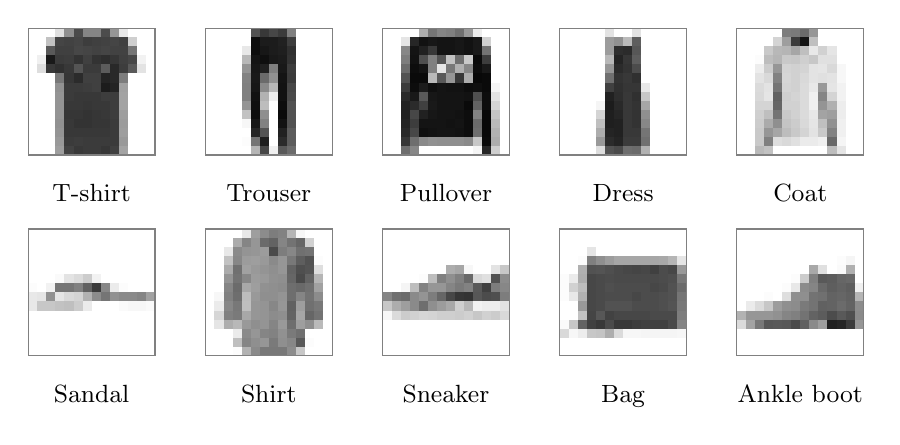
\begin{tikzpicture}
\fill[black!12] (0.345,1.495) rectangle ++(0.115,0.115);
\fill[black!44] (0.460,1.495) rectangle ++(0.115,0.115);
\fill[black!71] (0.575,1.495) rectangle ++(0.115,0.115);
\fill[black!48] (0.690,1.495) rectangle ++(0.115,0.115);
\fill[black!48] (0.805,1.495) rectangle ++(0.115,0.115);
\fill[black!70] (0.920,1.495) rectangle ++(0.115,0.115);
\fill[black!41] (1.035,1.495) rectangle ++(0.115,0.115);
\fill[black!9] (1.150,1.495) rectangle ++(0.115,0.115);
\fill[black!24] (0.230,1.380) rectangle ++(0.115,0.115);
\fill[black!73] (0.345,1.380) rectangle ++(0.115,0.115);
\fill[black!74] (0.460,1.380) rectangle ++(0.115,0.115);
\fill[black!73] (0.575,1.380) rectangle ++(0.115,0.115);
\fill[black!76] (0.690,1.380) rectangle ++(0.115,0.115);
\fill[black!75] (0.805,1.380) rectangle ++(0.115,0.115);
\fill[black!74] (0.920,1.380) rectangle ++(0.115,0.115);
\fill[black!73] (1.035,1.380) rectangle ++(0.115,0.115);
\fill[black!75] (1.150,1.380) rectangle ++(0.115,0.115);
\fill[black!19] (1.265,1.380) rectangle ++(0.115,0.115);
\fill[black!65] (0.230,1.265) rectangle ++(0.115,0.115);
\fill[black!75] (0.345,1.265) rectangle ++(0.115,0.115);
\fill[black!75] (0.460,1.265) rectangle ++(0.115,0.115);
\fill[black!72] (0.575,1.265) rectangle ++(0.115,0.115);
\fill[black!73] (0.690,1.265) rectangle ++(0.115,0.115);
\fill[black!74] (0.805,1.265) rectangle ++(0.115,0.115);
\fill[black!73] (0.920,1.265) rectangle ++(0.115,0.115);
\fill[black!74] (1.035,1.265) rectangle ++(0.115,0.115);
\fill[black!74] (1.150,1.265) rectangle ++(0.115,0.115);
\fill[black!54] (1.265,1.265) rectangle ++(0.115,0.115);
\fill[black!6] (0.115,1.150) rectangle ++(0.115,0.115);
\fill[black!90] (0.230,1.150) rectangle ++(0.115,0.115);
\fill[black!77] (0.345,1.150) rectangle ++(0.115,0.115);
\fill[black!76] (0.460,1.150) rectangle ++(0.115,0.115);
\fill[black!80] (0.575,1.150) rectangle ++(0.115,0.115);
\fill[black!75] (0.690,1.150) rectangle ++(0.115,0.115);
\fill[black!80] (0.805,1.150) rectangle ++(0.115,0.115);
\fill[black!82] (0.920,1.150) rectangle ++(0.115,0.115);
\fill[black!79] (1.035,1.150) rectangle ++(0.115,0.115);
\fill[black!75] (1.150,1.150) rectangle ++(0.115,0.115);
\fill[black!72] (1.265,1.150) rectangle ++(0.115,0.115);
\fill[black!5] (1.380,1.150) rectangle ++(0.115,0.115);
\fill[black!13] (0.115,1.035) rectangle ++(0.115,0.115);
\fill[black!78] (0.230,1.035) rectangle ++(0.115,0.115);
\fill[black!81] (0.345,1.035) rectangle ++(0.115,0.115);
\fill[black!78] (0.460,1.035) rectangle ++(0.115,0.115);
\fill[black!67] (0.575,1.035) rectangle ++(0.115,0.115);
\fill[black!77] (0.690,1.035) rectangle ++(0.115,0.115);
\fill[black!77] (0.805,1.035) rectangle ++(0.115,0.115);
\fill[black!64] (0.920,1.035) rectangle ++(0.115,0.115);
\fill[black!84] (1.035,1.035) rectangle ++(0.115,0.115);
\fill[black!76] (1.150,1.035) rectangle ++(0.115,0.115);
\fill[black!65] (1.265,1.035) rectangle ++(0.115,0.115);
\fill[black!11] (1.380,1.035) rectangle ++(0.115,0.115);
\fill[black!53] (0.345,0.920) rectangle ++(0.115,0.115);
\fill[black!79] (0.460,0.920) rectangle ++(0.115,0.115);
\fill[black!83] (0.575,0.920) rectangle ++(0.115,0.115);
\fill[black!75] (0.690,0.920) rectangle ++(0.115,0.115);
\fill[black!75] (0.805,0.920) rectangle ++(0.115,0.115);
\fill[black!86] (0.920,0.920) rectangle ++(0.115,0.115);
\fill[black!84] (1.035,0.920) rectangle ++(0.115,0.115);
\fill[black!51] (1.150,0.920) rectangle ++(0.115,0.115);
\fill[black!43] (0.345,0.805) rectangle ++(0.115,0.115);
\fill[black!77] (0.460,0.805) rectangle ++(0.115,0.115);
\fill[black!77] (0.575,0.805) rectangle ++(0.115,0.115);
\fill[black!76] (0.690,0.805) rectangle ++(0.115,0.115);
\fill[black!75] (0.805,0.805) rectangle ++(0.115,0.115);
\fill[black!89] (0.920,0.805) rectangle ++(0.115,0.115);
\fill[black!86] (1.035,0.805) rectangle ++(0.115,0.115);
\fill[black!37] (1.150,0.805) rectangle ++(0.115,0.115);
\fill[black!42] (0.345,0.690) rectangle ++(0.115,0.115);
\fill[black!77] (0.460,0.690) rectangle ++(0.115,0.115);
\fill[black!78] (0.575,0.690) rectangle ++(0.115,0.115);
\fill[black!78] (0.690,0.690) rectangle ++(0.115,0.115);
\fill[black!78] (0.805,0.690) rectangle ++(0.115,0.115);
\fill[black!76] (0.920,0.690) rectangle ++(0.115,0.115);
\fill[black!76] (1.035,0.690) rectangle ++(0.115,0.115);
\fill[black!36] (1.150,0.690) rectangle ++(0.115,0.115);
\fill[black!42] (0.345,0.575) rectangle ++(0.115,0.115);
\fill[black!78] (0.460,0.575) rectangle ++(0.115,0.115);
\fill[black!78] (0.575,0.575) rectangle ++(0.115,0.115);
\fill[black!79] (0.690,0.575) rectangle ++(0.115,0.115);
\fill[black!78] (0.805,0.575) rectangle ++(0.115,0.115);
\fill[black!78] (0.920,0.575) rectangle ++(0.115,0.115);
\fill[black!76] (1.035,0.575) rectangle ++(0.115,0.115);
\fill[black!36] (1.150,0.575) rectangle ++(0.115,0.115);
\fill[black!42] (0.345,0.460) rectangle ++(0.115,0.115);
\fill[black!79] (0.460,0.460) rectangle ++(0.115,0.115);
\fill[black!79] (0.575,0.460) rectangle ++(0.115,0.115);
\fill[black!80] (0.690,0.460) rectangle ++(0.115,0.115);
\fill[black!79] (0.805,0.460) rectangle ++(0.115,0.115);
\fill[black!78] (0.920,0.460) rectangle ++(0.115,0.115);
\fill[black!76] (1.035,0.460) rectangle ++(0.115,0.115);
\fill[black!38] (1.150,0.460) rectangle ++(0.115,0.115);
\fill[black!43] (0.345,0.345) rectangle ++(0.115,0.115);
\fill[black!78] (0.460,0.345) rectangle ++(0.115,0.115);
\fill[black!80] (0.575,0.345) rectangle ++(0.115,0.115);
\fill[black!80] (0.690,0.345) rectangle ++(0.115,0.115);
\fill[black!79] (0.805,0.345) rectangle ++(0.115,0.115);
\fill[black!79] (0.920,0.345) rectangle ++(0.115,0.115);
\fill[black!77] (1.035,0.345) rectangle ++(0.115,0.115);
\fill[black!39] (1.150,0.345) rectangle ++(0.115,0.115);
\fill[black!42] (0.345,0.230) rectangle ++(0.115,0.115);
\fill[black!78] (0.460,0.230) rectangle ++(0.115,0.115);
\fill[black!78] (0.575,0.230) rectangle ++(0.115,0.115);
\fill[black!78] (0.690,0.230) rectangle ++(0.115,0.115);
\fill[black!78] (0.805,0.230) rectangle ++(0.115,0.115);
\fill[black!78] (0.920,0.230) rectangle ++(0.115,0.115);
\fill[black!77] (1.035,0.230) rectangle ++(0.115,0.115);
\fill[black!38] (1.150,0.230) rectangle ++(0.115,0.115);
\fill[black!40] (0.345,0.115) rectangle ++(0.115,0.115);
\fill[black!77] (0.460,0.115) rectangle ++(0.115,0.115);
\fill[black!76] (0.575,0.115) rectangle ++(0.115,0.115);
\fill[black!77] (0.690,0.115) rectangle ++(0.115,0.115);
\fill[black!77] (0.805,0.115) rectangle ++(0.115,0.115);
\fill[black!77] (0.920,0.115) rectangle ++(0.115,0.115);
\fill[black!77] (1.035,0.115) rectangle ++(0.115,0.115);
\fill[black!40] (1.150,0.115) rectangle ++(0.115,0.115);
\fill[black!38] (0.345,0.000) rectangle ++(0.115,0.115);
\fill[black!74] (0.460,0.000) rectangle ++(0.115,0.115);
\fill[black!78] (0.575,0.000) rectangle ++(0.115,0.115);
\fill[black!77] (0.690,0.000) rectangle ++(0.115,0.115);
\fill[black!77] (0.805,0.000) rectangle ++(0.115,0.115);
\fill[black!79] (0.920,0.000) rectangle ++(0.115,0.115);
\fill[black!75] (1.035,0.000) rectangle ++(0.115,0.115);
\fill[black!36] (1.150,0.000) rectangle ++(0.115,0.115);
\draw[gray] (0.0,0.0) rectangle (1.610,1.610);
\fill[black!68] (2.825,1.495) rectangle ++(0.115,0.115);
\fill[black!78] (2.940,1.495) rectangle ++(0.115,0.115);
\fill[black!72] (3.055,1.495) rectangle ++(0.115,0.115);
\fill[black!77] (3.170,1.495) rectangle ++(0.115,0.115);
\fill[black!50] (3.285,1.495) rectangle ++(0.115,0.115);
\fill[black!95] (2.825,1.380) rectangle ++(0.115,0.115);
\fill[black!89] (2.940,1.380) rectangle ++(0.115,0.115);
\fill[black!89] (3.055,1.380) rectangle ++(0.115,0.115);
\fill[black!87] (3.170,1.380) rectangle ++(0.115,0.115);
\fill[black!76] (3.285,1.380) rectangle ++(0.115,0.115);
\fill[black!9] (2.710,1.265) rectangle ++(0.115,0.115);
\fill[black!95] (2.825,1.265) rectangle ++(0.115,0.115);
\fill[black!91] (2.940,1.265) rectangle ++(0.115,0.115);
\fill[black!89] (3.055,1.265) rectangle ++(0.115,0.115);
\fill[black!88] (3.170,1.265) rectangle ++(0.115,0.115);
\fill[black!81] (3.285,1.265) rectangle ++(0.115,0.115);
\fill[black!28] (2.710,1.150) rectangle ++(0.115,0.115);
\fill[black!92] (2.825,1.150) rectangle ++(0.115,0.115);
\fill[black!94] (2.940,1.150) rectangle ++(0.115,0.115);
\fill[black!90] (3.055,1.150) rectangle ++(0.115,0.115);
\fill[black!89] (3.170,1.150) rectangle ++(0.115,0.115);
\fill[black!80] (3.285,1.150) rectangle ++(0.115,0.115);
\fill[black!42] (2.710,1.035) rectangle ++(0.115,0.115);
\fill[black!91] (2.825,1.035) rectangle ++(0.115,0.115);
\fill[black!87] (2.940,1.035) rectangle ++(0.115,0.115);
\fill[black!50] (3.055,1.035) rectangle ++(0.115,0.115);
\fill[black!90] (3.170,1.035) rectangle ++(0.115,0.115);
\fill[black!76] (3.285,1.035) rectangle ++(0.115,0.115);
\fill[black!49] (2.710,0.920) rectangle ++(0.115,0.115);
\fill[black!90] (2.825,0.920) rectangle ++(0.115,0.115);
\fill[black!58] (2.940,0.920) rectangle ++(0.115,0.115);
\fill[black!43] (3.055,0.920) rectangle ++(0.115,0.115);
\fill[black!92] (3.170,0.920) rectangle ++(0.115,0.115);
\fill[black!77] (3.285,0.920) rectangle ++(0.115,0.115);
\fill[black!50] (2.710,0.805) rectangle ++(0.115,0.115);
\fill[black!91] (2.825,0.805) rectangle ++(0.115,0.115);
\fill[black!46] (2.940,0.805) rectangle ++(0.115,0.115);
\fill[black!28] (3.055,0.805) rectangle ++(0.115,0.115);
\fill[black!93] (3.170,0.805) rectangle ++(0.115,0.115);
\fill[black!72] (3.285,0.805) rectangle ++(0.115,0.115);
\fill[black!50] (2.710,0.690) rectangle ++(0.115,0.115);
\fill[black!93] (2.825,0.690) rectangle ++(0.115,0.115);
\fill[black!30] (2.940,0.690) rectangle ++(0.115,0.115);
\fill[black!7] (3.055,0.690) rectangle ++(0.115,0.115);
\fill[black!93] (3.170,0.690) rectangle ++(0.115,0.115);
\fill[black!71] (3.285,0.690) rectangle ++(0.115,0.115);
\fill[black!42] (2.710,0.575) rectangle ++(0.115,0.115);
\fill[black!94] (2.825,0.575) rectangle ++(0.115,0.115);
\fill[black!26] (2.940,0.575) rectangle ++(0.115,0.115);
\fill[black!1] (3.055,0.575) rectangle ++(0.115,0.115);
\fill[black!95] (3.170,0.575) rectangle ++(0.115,0.115);
\fill[black!68] (3.285,0.575) rectangle ++(0.115,0.115);
\fill[black!24] (2.710,0.460) rectangle ++(0.115,0.115);
\fill[black!95] (2.825,0.460) rectangle ++(0.115,0.115);
\fill[black!44] (2.940,0.460) rectangle ++(0.115,0.115);
\fill[black!96] (3.170,0.460) rectangle ++(0.115,0.115);
\fill[black!68] (3.285,0.460) rectangle ++(0.115,0.115);
\fill[black!3] (2.710,0.345) rectangle ++(0.115,0.115);
\fill[black!91] (2.825,0.345) rectangle ++(0.115,0.115);
\fill[black!49] (2.940,0.345) rectangle ++(0.115,0.115);
\fill[black!93] (3.170,0.345) rectangle ++(0.115,0.115);
\fill[black!68] (3.285,0.345) rectangle ++(0.115,0.115);
\fill[black!85] (2.825,0.230) rectangle ++(0.115,0.115);
\fill[black!67] (2.940,0.230) rectangle ++(0.115,0.115);
\fill[black!87] (3.170,0.230) rectangle ++(0.115,0.115);
\fill[black!64] (3.285,0.230) rectangle ++(0.115,0.115);
\fill[black!1] (2.710,0.115) rectangle ++(0.115,0.115);
\fill[black!54] (2.825,0.115) rectangle ++(0.115,0.115);
\fill[black!88] (2.940,0.115) rectangle ++(0.115,0.115);
\fill[black!83] (3.170,0.115) rectangle ++(0.115,0.115);
\fill[black!64] (3.285,0.115) rectangle ++(0.115,0.115);
\fill[black!29] (2.825,0.000) rectangle ++(0.115,0.115);
\fill[black!72] (2.940,0.000) rectangle ++(0.115,0.115);
\fill[black!6] (3.055,0.000) rectangle ++(0.115,0.115);
\fill[black!65] (3.170,0.000) rectangle ++(0.115,0.115);
\fill[black!58] (3.285,0.000) rectangle ++(0.115,0.115);
\draw[gray] (2.25,0.0) rectangle (3.860,1.610);
\fill[black!1] (4.845,1.495) rectangle ++(0.115,0.115);
\fill[black!32] (4.960,1.495) rectangle ++(0.115,0.115);
\fill[black!54] (5.075,1.495) rectangle ++(0.115,0.115);
\fill[black!48] (5.190,1.495) rectangle ++(0.115,0.115);
\fill[black!50] (5.305,1.495) rectangle ++(0.115,0.115);
\fill[black!56] (5.420,1.495) rectangle ++(0.115,0.115);
\fill[black!40] (5.535,1.495) rectangle ++(0.115,0.115);
\fill[black!7] (5.650,1.495) rectangle ++(0.115,0.115);
\fill[black!10] (4.730,1.380) rectangle ++(0.115,0.115);
\fill[black!85] (4.845,1.380) rectangle ++(0.115,0.115);
\fill[black!93] (4.960,1.380) rectangle ++(0.115,0.115);
\fill[black!91] (5.075,1.380) rectangle ++(0.115,0.115);
\fill[black!92] (5.190,1.380) rectangle ++(0.115,0.115);
\fill[black!92] (5.305,1.380) rectangle ++(0.115,0.115);
\fill[black!91] (5.420,1.380) rectangle ++(0.115,0.115);
\fill[black!93] (5.535,1.380) rectangle ++(0.115,0.115);
\fill[black!90] (5.650,1.380) rectangle ++(0.115,0.115);
\fill[black!18] (5.765,1.380) rectangle ++(0.115,0.115);
\fill[black!47] (4.730,1.265) rectangle ++(0.115,0.115);
\fill[black!92] (4.845,1.265) rectangle ++(0.115,0.115);
\fill[black!87] (4.960,1.265) rectangle ++(0.115,0.115);
\fill[black!78] (5.075,1.265) rectangle ++(0.115,0.115);
\fill[black!92] (5.190,1.265) rectangle ++(0.115,0.115);
\fill[black!92] (5.305,1.265) rectangle ++(0.115,0.115);
\fill[black!91] (5.420,1.265) rectangle ++(0.115,0.115);
\fill[black!93] (5.535,1.265) rectangle ++(0.115,0.115);
\fill[black!90] (5.650,1.265) rectangle ++(0.115,0.115);
\fill[black!55] (5.765,1.265) rectangle ++(0.115,0.115);
\fill[black!51] (4.730,1.150) rectangle ++(0.115,0.115);
\fill[black!93] (4.845,1.150) rectangle ++(0.115,0.115);
\fill[black!69] (4.960,1.150) rectangle ++(0.115,0.115);
\fill[black!50] (5.075,1.150) rectangle ++(0.115,0.115);
\fill[black!67] (5.190,1.150) rectangle ++(0.115,0.115);
\fill[black!24] (5.305,1.150) rectangle ++(0.115,0.115);
\fill[black!57] (5.420,1.150) rectangle ++(0.115,0.115);
\fill[black!21] (5.535,1.150) rectangle ++(0.115,0.115);
\fill[black!96] (5.650,1.150) rectangle ++(0.115,0.115);
\fill[black!76] (5.765,1.150) rectangle ++(0.115,0.115);
\fill[black!58] (4.730,1.035) rectangle ++(0.115,0.115);
\fill[black!95] (4.845,1.035) rectangle ++(0.115,0.115);
\fill[black!92] (4.960,1.035) rectangle ++(0.115,0.115);
\fill[black!50] (5.075,1.035) rectangle ++(0.115,0.115);
\fill[black!10] (5.190,1.035) rectangle ++(0.115,0.115);
\fill[black!53] (5.305,1.035) rectangle ++(0.115,0.115);
\fill[black!31] (5.420,1.035) rectangle ++(0.115,0.115);
\fill[black!47] (5.535,1.035) rectangle ++(0.115,0.115);
\fill[black!95] (5.650,1.035) rectangle ++(0.115,0.115);
\fill[black!90] (5.765,1.035) rectangle ++(0.115,0.115);
\fill[black!68] (4.730,0.920) rectangle ++(0.115,0.115);
\fill[black!96] (4.845,0.920) rectangle ++(0.115,0.115);
\fill[black!96] (4.960,0.920) rectangle ++(0.115,0.115);
\fill[black!27] (5.075,0.920) rectangle ++(0.115,0.115);
\fill[black!65] (5.190,0.920) rectangle ++(0.115,0.115);
\fill[black!41] (5.305,0.920) rectangle ++(0.115,0.115);
\fill[black!78] (5.420,0.920) rectangle ++(0.115,0.115);
\fill[black!32] (5.535,0.920) rectangle ++(0.115,0.115);
\fill[black!97] (5.650,0.920) rectangle ++(0.115,0.115);
\fill[black!96] (5.765,0.920) rectangle ++(0.115,0.115);
\fill[black!77] (4.730,0.805) rectangle ++(0.115,0.115);
\fill[black!95] (4.845,0.805) rectangle ++(0.115,0.115);
\fill[black!89] (4.960,0.805) rectangle ++(0.115,0.115);
\fill[black!94] (5.075,0.805) rectangle ++(0.115,0.115);
\fill[black!92] (5.190,0.805) rectangle ++(0.115,0.115);
\fill[black!93] (5.305,0.805) rectangle ++(0.115,0.115);
\fill[black!93] (5.420,0.805) rectangle ++(0.115,0.115);
\fill[black!95] (5.535,0.805) rectangle ++(0.115,0.115);
\fill[black!94] (5.650,0.805) rectangle ++(0.115,0.115);
\fill[black!96] (5.765,0.805) rectangle ++(0.115,0.115);
\fill[black!4] (5.880,0.805) rectangle ++(0.115,0.115);
\fill[black!84] (4.730,0.690) rectangle ++(0.115,0.115);
\fill[black!90] (4.845,0.690) rectangle ++(0.115,0.115);
\fill[black!65] (4.960,0.690) rectangle ++(0.115,0.115);
\fill[black!91] (5.075,0.690) rectangle ++(0.115,0.115);
\fill[black!92] (5.190,0.690) rectangle ++(0.115,0.115);
\fill[black!92] (5.305,0.690) rectangle ++(0.115,0.115);
\fill[black!92] (5.420,0.690) rectangle ++(0.115,0.115);
\fill[black!93] (5.535,0.690) rectangle ++(0.115,0.115);
\fill[black!69] (5.650,0.690) rectangle ++(0.115,0.115);
\fill[black!95] (5.765,0.690) rectangle ++(0.115,0.115);
\fill[black!11] (5.880,0.690) rectangle ++(0.115,0.115);
\fill[black!87] (4.730,0.575) rectangle ++(0.115,0.115);
\fill[black!83] (4.845,0.575) rectangle ++(0.115,0.115);
\fill[black!75] (4.960,0.575) rectangle ++(0.115,0.115);
\fill[black!90] (5.075,0.575) rectangle ++(0.115,0.115);
\fill[black!92] (5.190,0.575) rectangle ++(0.115,0.115);
\fill[black!92] (5.305,0.575) rectangle ++(0.115,0.115);
\fill[black!92] (5.420,0.575) rectangle ++(0.115,0.115);
\fill[black!96] (5.535,0.575) rectangle ++(0.115,0.115);
\fill[black!61] (5.650,0.575) rectangle ++(0.115,0.115);
\fill[black!95] (5.765,0.575) rectangle ++(0.115,0.115);
\fill[black!17] (5.880,0.575) rectangle ++(0.115,0.115);
\fill[black!87] (4.730,0.460) rectangle ++(0.115,0.115);
\fill[black!72] (4.845,0.460) rectangle ++(0.115,0.115);
\fill[black!87] (4.960,0.460) rectangle ++(0.115,0.115);
\fill[black!91] (5.075,0.460) rectangle ++(0.115,0.115);
\fill[black!92] (5.190,0.460) rectangle ++(0.115,0.115);
\fill[black!92] (5.305,0.460) rectangle ++(0.115,0.115);
\fill[black!93] (5.420,0.460) rectangle ++(0.115,0.115);
\fill[black!95] (5.535,0.460) rectangle ++(0.115,0.115);
\fill[black!49] (5.650,0.460) rectangle ++(0.115,0.115);
\fill[black!97] (5.765,0.460) rectangle ++(0.115,0.115);
\fill[black!23] (5.880,0.460) rectangle ++(0.115,0.115);
\fill[black!86] (4.730,0.345) rectangle ++(0.115,0.115);
\fill[black!76] (4.845,0.345) rectangle ++(0.115,0.115);
\fill[black!92] (4.960,0.345) rectangle ++(0.115,0.115);
\fill[black!92] (5.075,0.345) rectangle ++(0.115,0.115);
\fill[black!92] (5.190,0.345) rectangle ++(0.115,0.115);
\fill[black!93] (5.305,0.345) rectangle ++(0.115,0.115);
\fill[black!92] (5.420,0.345) rectangle ++(0.115,0.115);
\fill[black!95] (5.535,0.345) rectangle ++(0.115,0.115);
\fill[black!58] (5.650,0.345) rectangle ++(0.115,0.115);
\fill[black!97] (5.765,0.345) rectangle ++(0.115,0.115);
\fill[black!27] (5.880,0.345) rectangle ++(0.115,0.115);
\fill[black!84] (4.730,0.230) rectangle ++(0.115,0.115);
\fill[black!72] (4.845,0.230) rectangle ++(0.115,0.115);
\fill[black!94] (4.960,0.230) rectangle ++(0.115,0.115);
\fill[black!93] (5.075,0.230) rectangle ++(0.115,0.115);
\fill[black!92] (5.190,0.230) rectangle ++(0.115,0.115);
\fill[black!92] (5.305,0.230) rectangle ++(0.115,0.115);
\fill[black!93] (5.420,0.230) rectangle ++(0.115,0.115);
\fill[black!95] (5.535,0.230) rectangle ++(0.115,0.115);
\fill[black!57] (5.650,0.230) rectangle ++(0.115,0.115);
\fill[black!97] (5.765,0.230) rectangle ++(0.115,0.115);
\fill[black!30] (5.880,0.230) rectangle ++(0.115,0.115);
\fill[black!79] (4.730,0.115) rectangle ++(0.115,0.115);
\fill[black!57] (4.845,0.115) rectangle ++(0.115,0.115);
\fill[black!46] (4.960,0.115) rectangle ++(0.115,0.115);
\fill[black!43] (5.075,0.115) rectangle ++(0.115,0.115);
\fill[black!44] (5.190,0.115) rectangle ++(0.115,0.115);
\fill[black!44] (5.305,0.115) rectangle ++(0.115,0.115);
\fill[black!44] (5.420,0.115) rectangle ++(0.115,0.115);
\fill[black!46] (5.535,0.115) rectangle ++(0.115,0.115);
\fill[black!22] (5.650,0.115) rectangle ++(0.115,0.115);
\fill[black!96] (5.765,0.115) rectangle ++(0.115,0.115);
\fill[black!32] (5.880,0.115) rectangle ++(0.115,0.115);
\fill[black!57] (4.730,0.000) rectangle ++(0.115,0.115);
\fill[black!47] (4.845,0.000) rectangle ++(0.115,0.115);
\fill[black!4] (5.650,0.000) rectangle ++(0.115,0.115);
\fill[black!85] (5.765,0.000) rectangle ++(0.115,0.115);
\fill[black!19] (5.880,0.000) rectangle ++(0.115,0.115);
\draw[gray] (4.5,0.0) rectangle (6.110,1.610);
\fill[black!11] (7.325,1.495) rectangle ++(0.115,0.115);
\fill[black!11] (7.670,1.495) rectangle ++(0.115,0.115);
\fill[black!39] (7.325,1.380) rectangle ++(0.115,0.115);
\fill[black!43] (7.440,1.380) rectangle ++(0.115,0.115);
\fill[black!27] (7.555,1.380) rectangle ++(0.115,0.115);
\fill[black!63] (7.670,1.380) rectangle ++(0.115,0.115);
\fill[black!39] (7.325,1.265) rectangle ++(0.115,0.115);
\fill[black!82] (7.440,1.265) rectangle ++(0.115,0.115);
\fill[black!83] (7.555,1.265) rectangle ++(0.115,0.115);
\fill[black!66] (7.670,1.265) rectangle ++(0.115,0.115);
\fill[black!28] (7.325,1.150) rectangle ++(0.115,0.115);
\fill[black!86] (7.440,1.150) rectangle ++(0.115,0.115);
\fill[black!79] (7.555,1.150) rectangle ++(0.115,0.115);
\fill[black!63] (7.670,1.150) rectangle ++(0.115,0.115);
\fill[black!41] (7.325,1.035) rectangle ++(0.115,0.115);
\fill[black!83] (7.440,1.035) rectangle ++(0.115,0.115);
\fill[black!80] (7.555,1.035) rectangle ++(0.115,0.115);
\fill[black!70] (7.670,1.035) rectangle ++(0.115,0.115);
\fill[black!56] (7.325,0.920) rectangle ++(0.115,0.115);
\fill[black!80] (7.440,0.920) rectangle ++(0.115,0.115);
\fill[black!78] (7.555,0.920) rectangle ++(0.115,0.115);
\fill[black!81] (7.670,0.920) rectangle ++(0.115,0.115);
\fill[black!75] (7.325,0.805) rectangle ++(0.115,0.115);
\fill[black!81] (7.440,0.805) rectangle ++(0.115,0.115);
\fill[black!79] (7.555,0.805) rectangle ++(0.115,0.115);
\fill[black!79] (7.670,0.805) rectangle ++(0.115,0.115);
\fill[black!9] (7.785,0.805) rectangle ++(0.115,0.115);
\fill[black!87] (7.325,0.690) rectangle ++(0.115,0.115);
\fill[black!82] (7.440,0.690) rectangle ++(0.115,0.115);
\fill[black!78] (7.555,0.690) rectangle ++(0.115,0.115);
\fill[black!81] (7.670,0.690) rectangle ++(0.115,0.115);
\fill[black!22] (7.785,0.690) rectangle ++(0.115,0.115);
\fill[black!4] (7.210,0.575) rectangle ++(0.115,0.115);
\fill[black!89] (7.325,0.575) rectangle ++(0.115,0.115);
\fill[black!84] (7.440,0.575) rectangle ++(0.115,0.115);
\fill[black!78] (7.555,0.575) rectangle ++(0.115,0.115);
\fill[black!80] (7.670,0.575) rectangle ++(0.115,0.115);
\fill[black!35] (7.785,0.575) rectangle ++(0.115,0.115);
\fill[black!17] (7.210,0.460) rectangle ++(0.115,0.115);
\fill[black!88] (7.325,0.460) rectangle ++(0.115,0.115);
\fill[black!85] (7.440,0.460) rectangle ++(0.115,0.115);
\fill[black!78] (7.555,0.460) rectangle ++(0.115,0.115);
\fill[black!80] (7.670,0.460) rectangle ++(0.115,0.115);
\fill[black!44] (7.785,0.460) rectangle ++(0.115,0.115);
\fill[black!25] (7.210,0.345) rectangle ++(0.115,0.115);
\fill[black!88] (7.325,0.345) rectangle ++(0.115,0.115);
\fill[black!87] (7.440,0.345) rectangle ++(0.115,0.115);
\fill[black!78] (7.555,0.345) rectangle ++(0.115,0.115);
\fill[black!80] (7.670,0.345) rectangle ++(0.115,0.115);
\fill[black!47] (7.785,0.345) rectangle ++(0.115,0.115);
\fill[black!32] (7.210,0.230) rectangle ++(0.115,0.115);
\fill[black!86] (7.325,0.230) rectangle ++(0.115,0.115);
\fill[black!87] (7.440,0.230) rectangle ++(0.115,0.115);
\fill[black!78] (7.555,0.230) rectangle ++(0.115,0.115);
\fill[black!78] (7.670,0.230) rectangle ++(0.115,0.115);
\fill[black!54] (7.785,0.230) rectangle ++(0.115,0.115);
\fill[black!40] (7.210,0.115) rectangle ++(0.115,0.115);
\fill[black!83] (7.325,0.115) rectangle ++(0.115,0.115);
\fill[black!86] (7.440,0.115) rectangle ++(0.115,0.115);
\fill[black!77] (7.555,0.115) rectangle ++(0.115,0.115);
\fill[black!77] (7.670,0.115) rectangle ++(0.115,0.115);
\fill[black!56] (7.785,0.115) rectangle ++(0.115,0.115);
\fill[black!13] (7.210,0.000) rectangle ++(0.115,0.115);
\fill[black!68] (7.325,0.000) rectangle ++(0.115,0.115);
\fill[black!71] (7.440,0.000) rectangle ++(0.115,0.115);
\fill[black!57] (7.555,0.000) rectangle ++(0.115,0.115);
\fill[black!58] (7.670,0.000) rectangle ++(0.115,0.115);
\fill[black!30] (7.785,0.000) rectangle ++(0.115,0.115);
\draw[gray] (6.75,0.0) rectangle (8.360,1.610);
\fill[black!51] (9.575,1.495) rectangle ++(0.115,0.115);
\fill[black!52] (9.690,1.495) rectangle ++(0.115,0.115);
\fill[black!58] (9.805,1.495) rectangle ++(0.115,0.115);
\fill[black!41] (9.920,1.495) rectangle ++(0.115,0.115);
\fill[black!17] (9.460,1.380) rectangle ++(0.115,0.115);
\fill[black!38] (9.575,1.380) rectangle ++(0.115,0.115);
\fill[black!77] (9.690,1.380) rectangle ++(0.115,0.115);
\fill[black!92] (9.805,1.380) rectangle ++(0.115,0.115);
\fill[black!25] (9.920,1.380) rectangle ++(0.115,0.115);
\fill[black!21] (9.345,1.265) rectangle ++(0.115,0.115);
\fill[black!28] (9.460,1.265) rectangle ++(0.115,0.115);
\fill[black!29] (9.575,1.265) rectangle ++(0.115,0.115);
\fill[black!35] (9.690,1.265) rectangle ++(0.115,0.115);
\fill[black!25] (9.805,1.265) rectangle ++(0.115,0.115);
\fill[black!9] (9.920,1.265) rectangle ++(0.115,0.115);
\fill[black!18] (10.035,1.265) rectangle ++(0.115,0.115);
\fill[black!10] (10.150,1.265) rectangle ++(0.115,0.115);
\fill[black!1] (9.230,1.150) rectangle ++(0.115,0.115);
\fill[black!26] (9.345,1.150) rectangle ++(0.115,0.115);
\fill[black!29] (9.460,1.150) rectangle ++(0.115,0.115);
\fill[black!21] (9.575,1.150) rectangle ++(0.115,0.115);
\fill[black!22] (9.690,1.150) rectangle ++(0.115,0.115);
\fill[black!19] (9.805,1.150) rectangle ++(0.115,0.115);
\fill[black!22] (9.920,1.150) rectangle ++(0.115,0.115);
\fill[black!12] (10.035,1.150) rectangle ++(0.115,0.115);
\fill[black!12] (10.150,1.150) rectangle ++(0.115,0.115);
\fill[black!7] (9.230,1.035) rectangle ++(0.115,0.115);
\fill[black!20] (9.345,1.035) rectangle ++(0.115,0.115);
\fill[black!41] (9.460,1.035) rectangle ++(0.115,0.115);
\fill[black!17] (9.575,1.035) rectangle ++(0.115,0.115);
\fill[black!18] (9.690,1.035) rectangle ++(0.115,0.115);
\fill[black!17] (9.805,1.035) rectangle ++(0.115,0.115);
\fill[black!11] (9.920,1.035) rectangle ++(0.115,0.115);
\fill[black!10] (10.035,1.035) rectangle ++(0.115,0.115);
\fill[black!15] (10.150,1.035) rectangle ++(0.115,0.115);
\fill[black!3] (10.265,1.035) rectangle ++(0.115,0.115);
\fill[black!11] (9.230,0.920) rectangle ++(0.115,0.115);
\fill[black!15] (9.345,0.920) rectangle ++(0.115,0.115);
\fill[black!49] (9.460,0.920) rectangle ++(0.115,0.115);
\fill[black!16] (9.575,0.920) rectangle ++(0.115,0.115);
\fill[black!18] (9.690,0.920) rectangle ++(0.115,0.115);
\fill[black!15] (9.805,0.920) rectangle ++(0.115,0.115);
\fill[black!11] (9.920,0.920) rectangle ++(0.115,0.115);
\fill[black!12] (10.035,0.920) rectangle ++(0.115,0.115);
\fill[black!11] (10.150,0.920) rectangle ++(0.115,0.115);
\fill[black!3] (10.265,0.920) rectangle ++(0.115,0.115);
\fill[black!14] (9.230,0.805) rectangle ++(0.115,0.115);
\fill[black!11] (9.345,0.805) rectangle ++(0.115,0.115);
\fill[black!54] (9.460,0.805) rectangle ++(0.115,0.115);
\fill[black!17] (9.575,0.805) rectangle ++(0.115,0.115);
\fill[black!18] (9.690,0.805) rectangle ++(0.115,0.115);
\fill[black!14] (9.805,0.805) rectangle ++(0.115,0.115);
\fill[black!9] (9.920,0.805) rectangle ++(0.115,0.115);
\fill[black!40] (10.035,0.805) rectangle ++(0.115,0.115);
\fill[black!10] (10.150,0.805) rectangle ++(0.115,0.115);
\fill[black!5] (10.265,0.805) rectangle ++(0.115,0.115);
\fill[black!15] (9.230,0.690) rectangle ++(0.115,0.115);
\fill[black!10] (9.345,0.690) rectangle ++(0.115,0.115);
\fill[black!62] (9.460,0.690) rectangle ++(0.115,0.115);
\fill[black!19] (9.575,0.690) rectangle ++(0.115,0.115);
\fill[black!17] (9.690,0.690) rectangle ++(0.115,0.115);
\fill[black!14] (9.805,0.690) rectangle ++(0.115,0.115);
\fill[black!6] (9.920,0.690) rectangle ++(0.115,0.115);
\fill[black!48] (10.035,0.690) rectangle ++(0.115,0.115);
\fill[black!17] (10.150,0.690) rectangle ++(0.115,0.115);
\fill[black!5] (10.265,0.690) rectangle ++(0.115,0.115);
\fill[black!17] (9.230,0.575) rectangle ++(0.115,0.115);
\fill[black!17] (9.345,0.575) rectangle ++(0.115,0.115);
\fill[black!60] (9.460,0.575) rectangle ++(0.115,0.115);
\fill[black!18] (9.575,0.575) rectangle ++(0.115,0.115);
\fill[black!18] (9.690,0.575) rectangle ++(0.115,0.115);
\fill[black!14] (9.805,0.575) rectangle ++(0.115,0.115);
\fill[black!6] (9.920,0.575) rectangle ++(0.115,0.115);
\fill[black!42] (10.035,0.575) rectangle ++(0.115,0.115);
\fill[black!31] (10.150,0.575) rectangle ++(0.115,0.115);
\fill[black!7] (10.265,0.575) rectangle ++(0.115,0.115);
\fill[black!19] (9.230,0.460) rectangle ++(0.115,0.115);
\fill[black!25] (9.345,0.460) rectangle ++(0.115,0.115);
\fill[black!55] (9.460,0.460) rectangle ++(0.115,0.115);
\fill[black!21] (9.575,0.460) rectangle ++(0.115,0.115);
\fill[black!18] (9.690,0.460) rectangle ++(0.115,0.115);
\fill[black!14] (9.805,0.460) rectangle ++(0.115,0.115);
\fill[black!9] (9.920,0.460) rectangle ++(0.115,0.115);
\fill[black!36] (10.035,0.460) rectangle ++(0.115,0.115);
\fill[black!38] (10.150,0.460) rectangle ++(0.115,0.115);
\fill[black!7] (10.265,0.460) rectangle ++(0.115,0.115);
\fill[black!20] (9.230,0.345) rectangle ++(0.115,0.115);
\fill[black!33] (9.345,0.345) rectangle ++(0.115,0.115);
\fill[black!44] (9.460,0.345) rectangle ++(0.115,0.115);
\fill[black!23] (9.575,0.345) rectangle ++(0.115,0.115);
\fill[black!20] (9.690,0.345) rectangle ++(0.115,0.115);
\fill[black!15] (9.805,0.345) rectangle ++(0.115,0.115);
\fill[black!10] (9.920,0.345) rectangle ++(0.115,0.115);
\fill[black!25] (10.035,0.345) rectangle ++(0.115,0.115);
\fill[black!43] (10.150,0.345) rectangle ++(0.115,0.115);
\fill[black!6] (10.265,0.345) rectangle ++(0.115,0.115);
\fill[black!21] (9.230,0.230) rectangle ++(0.115,0.115);
\fill[black!41] (9.345,0.230) rectangle ++(0.115,0.115);
\fill[black!35] (9.460,0.230) rectangle ++(0.115,0.115);
\fill[black!26] (9.575,0.230) rectangle ++(0.115,0.115);
\fill[black!21] (9.690,0.230) rectangle ++(0.115,0.115);
\fill[black!17] (9.805,0.230) rectangle ++(0.115,0.115);
\fill[black!11] (9.920,0.230) rectangle ++(0.115,0.115);
\fill[black!21] (10.035,0.230) rectangle ++(0.115,0.115);
\fill[black!49] (10.150,0.230) rectangle ++(0.115,0.115);
\fill[black!6] (10.265,0.230) rectangle ++(0.115,0.115);
\fill[black!21] (9.230,0.115) rectangle ++(0.115,0.115);
\fill[black!50] (9.345,0.115) rectangle ++(0.115,0.115);
\fill[black!13] (9.460,0.115) rectangle ++(0.115,0.115);
\fill[black!15] (9.575,0.115) rectangle ++(0.115,0.115);
\fill[black!12] (9.690,0.115) rectangle ++(0.115,0.115);
\fill[black!8] (9.805,0.115) rectangle ++(0.115,0.115);
\fill[black!8] (9.920,0.115) rectangle ++(0.115,0.115);
\fill[black!6] (10.035,0.115) rectangle ++(0.115,0.115);
\fill[black!59] (10.150,0.115) rectangle ++(0.115,0.115);
\fill[black!4] (10.265,0.115) rectangle ++(0.115,0.115);
\fill[black!27] (9.230,0.000) rectangle ++(0.115,0.115);
\fill[black!24] (9.345,0.000) rectangle ++(0.115,0.115);
\fill[black!26] (10.150,0.000) rectangle ++(0.115,0.115);
\fill[black!10] (10.265,0.000) rectangle ++(0.115,0.115);
\draw[gray] (9.0,0.0) rectangle (10.610,1.610);
\fill[black!2] (0.345,-1.630) rectangle ++(0.115,0.115);
\fill[black!11] (0.460,-1.630) rectangle ++(0.115,0.115);
\fill[black!14] (0.575,-1.630) rectangle ++(0.115,0.115);
\fill[black!20] (0.690,-1.630) rectangle ++(0.115,0.115);
\fill[black!5] (0.805,-1.630) rectangle ++(0.115,0.115);
\fill[black!1] (0.000,-1.745) rectangle ++(0.115,0.115);
\fill[black!5] (0.230,-1.745) rectangle ++(0.115,0.115);
\fill[black!54] (0.345,-1.745) rectangle ++(0.115,0.115);
\fill[black!54] (0.460,-1.745) rectangle ++(0.115,0.115);
\fill[black!50] (0.575,-1.745) rectangle ++(0.115,0.115);
\fill[black!62] (0.690,-1.745) rectangle ++(0.115,0.115);
\fill[black!77] (0.805,-1.745) rectangle ++(0.115,0.115);
\fill[black!47] (0.920,-1.745) rectangle ++(0.115,0.115);
\fill[black!8] (1.035,-1.745) rectangle ++(0.115,0.115);
\fill[black!1] (1.150,-1.745) rectangle ++(0.115,0.115);
\fill[black!9] (0.000,-1.860) rectangle ++(0.115,0.115);
\fill[black!10] (0.115,-1.860) rectangle ++(0.115,0.115);
\fill[black!43] (0.230,-1.860) rectangle ++(0.115,0.115);
\fill[black!10] (0.345,-1.860) rectangle ++(0.115,0.115);
\fill[black!15] (0.460,-1.860) rectangle ++(0.115,0.115);
\fill[black!17] (0.575,-1.860) rectangle ++(0.115,0.115);
\fill[black!30] (0.690,-1.860) rectangle ++(0.115,0.115);
\fill[black!45] (0.805,-1.860) rectangle ++(0.115,0.115);
\fill[black!54] (0.920,-1.860) rectangle ++(0.115,0.115);
\fill[black!43] (1.035,-1.860) rectangle ++(0.115,0.115);
\fill[black!46] (1.150,-1.860) rectangle ++(0.115,0.115);
\fill[black!46] (1.265,-1.860) rectangle ++(0.115,0.115);
\fill[black!48] (1.380,-1.860) rectangle ++(0.115,0.115);
\fill[black!37] (1.495,-1.860) rectangle ++(0.115,0.115);
\fill[black!9] (0.000,-1.975) rectangle ++(0.115,0.115);
\fill[black!22] (0.115,-1.975) rectangle ++(0.115,0.115);
\fill[black!22] (0.230,-1.975) rectangle ++(0.115,0.115);
\fill[black!24] (0.345,-1.975) rectangle ++(0.115,0.115);
\fill[black!25] (0.460,-1.975) rectangle ++(0.115,0.115);
\fill[black!20] (0.575,-1.975) rectangle ++(0.115,0.115);
\fill[black!8] (0.690,-1.975) rectangle ++(0.115,0.115);
\fill[black!2] (1.150,-1.975) rectangle ++(0.115,0.115);
\fill[black!3] (1.265,-1.975) rectangle ++(0.115,0.115);
\fill[black!3] (1.380,-1.975) rectangle ++(0.115,0.115);
\fill[black!2] (1.495,-1.975) rectangle ++(0.115,0.115);
\draw[gray] (0.0,-2.55) rectangle (1.610,-0.940);
\fill[black!9] (2.710,-1.055) rectangle ++(0.115,0.115);
\fill[black!38] (2.825,-1.055) rectangle ++(0.115,0.115);
\fill[black!45] (2.940,-1.055) rectangle ++(0.115,0.115);
\fill[black!51] (3.055,-1.055) rectangle ++(0.115,0.115);
\fill[black!49] (3.170,-1.055) rectangle ++(0.115,0.115);
\fill[black!29] (3.285,-1.055) rectangle ++(0.115,0.115);
\fill[black!3] (3.400,-1.055) rectangle ++(0.115,0.115);
\fill[black!33] (2.595,-1.170) rectangle ++(0.115,0.115);
\fill[black!48] (2.710,-1.170) rectangle ++(0.115,0.115);
\fill[black!41] (2.825,-1.170) rectangle ++(0.115,0.115);
\fill[black!58] (2.940,-1.170) rectangle ++(0.115,0.115);
\fill[black!61] (3.055,-1.170) rectangle ++(0.115,0.115);
\fill[black!48] (3.170,-1.170) rectangle ++(0.115,0.115);
\fill[black!55] (3.285,-1.170) rectangle ++(0.115,0.115);
\fill[black!60] (3.400,-1.170) rectangle ++(0.115,0.115);
\fill[black!18] (3.515,-1.170) rectangle ++(0.115,0.115);
\fill[black!9] (2.480,-1.285) rectangle ++(0.115,0.115);
\fill[black!46] (2.595,-1.285) rectangle ++(0.115,0.115);
\fill[black!42] (2.710,-1.285) rectangle ++(0.115,0.115);
\fill[black!41] (2.825,-1.285) rectangle ++(0.115,0.115);
\fill[black!39] (2.940,-1.285) rectangle ++(0.115,0.115);
\fill[black!71] (3.055,-1.285) rectangle ++(0.115,0.115);
\fill[black!51] (3.170,-1.285) rectangle ++(0.115,0.115);
\fill[black!47] (3.285,-1.285) rectangle ++(0.115,0.115);
\fill[black!56] (3.400,-1.285) rectangle ++(0.115,0.115);
\fill[black!55] (3.515,-1.285) rectangle ++(0.115,0.115);
\fill[black!24] (2.480,-1.400) rectangle ++(0.115,0.115);
\fill[black!47] (2.595,-1.400) rectangle ++(0.115,0.115);
\fill[black!39] (2.710,-1.400) rectangle ++(0.115,0.115);
\fill[black!38] (2.825,-1.400) rectangle ++(0.115,0.115);
\fill[black!40] (2.940,-1.400) rectangle ++(0.115,0.115);
\fill[black!46] (3.055,-1.400) rectangle ++(0.115,0.115);
\fill[black!41] (3.170,-1.400) rectangle ++(0.115,0.115);
\fill[black!53] (3.285,-1.400) rectangle ++(0.115,0.115);
\fill[black!63] (3.400,-1.400) rectangle ++(0.115,0.115);
\fill[black!68] (3.515,-1.400) rectangle ++(0.115,0.115);
\fill[black!1] (3.630,-1.400) rectangle ++(0.115,0.115);
\fill[black!33] (2.480,-1.515) rectangle ++(0.115,0.115);
\fill[black!56] (2.595,-1.515) rectangle ++(0.115,0.115);
\fill[black!37] (2.710,-1.515) rectangle ++(0.115,0.115);
\fill[black!40] (2.825,-1.515) rectangle ++(0.115,0.115);
\fill[black!42] (2.940,-1.515) rectangle ++(0.115,0.115);
\fill[black!44] (3.055,-1.515) rectangle ++(0.115,0.115);
\fill[black!41] (3.170,-1.515) rectangle ++(0.115,0.115);
\fill[black!61] (3.285,-1.515) rectangle ++(0.115,0.115);
\fill[black!69] (3.400,-1.515) rectangle ++(0.115,0.115);
\fill[black!67] (3.515,-1.515) rectangle ++(0.115,0.115);
\fill[black!13] (3.630,-1.515) rectangle ++(0.115,0.115);
\fill[black!42] (2.480,-1.630) rectangle ++(0.115,0.115);
\fill[black!55] (2.595,-1.630) rectangle ++(0.115,0.115);
\fill[black!47] (2.710,-1.630) rectangle ++(0.115,0.115);
\fill[black!39] (2.825,-1.630) rectangle ++(0.115,0.115);
\fill[black!40] (2.940,-1.630) rectangle ++(0.115,0.115);
\fill[black!43] (3.055,-1.630) rectangle ++(0.115,0.115);
\fill[black!44] (3.170,-1.630) rectangle ++(0.115,0.115);
\fill[black!60] (3.285,-1.630) rectangle ++(0.115,0.115);
\fill[black!71] (3.400,-1.630) rectangle ++(0.115,0.115);
\fill[black!61] (3.515,-1.630) rectangle ++(0.115,0.115);
\fill[black!29] (3.630,-1.630) rectangle ++(0.115,0.115);
\fill[black!48] (2.480,-1.745) rectangle ++(0.115,0.115);
\fill[black!58] (2.595,-1.745) rectangle ++(0.115,0.115);
\fill[black!34] (2.710,-1.745) rectangle ++(0.115,0.115);
\fill[black!38] (2.825,-1.745) rectangle ++(0.115,0.115);
\fill[black!43] (2.940,-1.745) rectangle ++(0.115,0.115);
\fill[black!44] (3.055,-1.745) rectangle ++(0.115,0.115);
\fill[black!45] (3.170,-1.745) rectangle ++(0.115,0.115);
\fill[black!57] (3.285,-1.745) rectangle ++(0.115,0.115);
\fill[black!59] (3.400,-1.745) rectangle ++(0.115,0.115);
\fill[black!56] (3.515,-1.745) rectangle ++(0.115,0.115);
\fill[black!37] (3.630,-1.745) rectangle ++(0.115,0.115);
\fill[black!3] (2.365,-1.860) rectangle ++(0.115,0.115);
\fill[black!50] (2.480,-1.860) rectangle ++(0.115,0.115);
\fill[black!57] (2.595,-1.860) rectangle ++(0.115,0.115);
\fill[black!26] (2.710,-1.860) rectangle ++(0.115,0.115);
\fill[black!40] (2.825,-1.860) rectangle ++(0.115,0.115);
\fill[black!44] (2.940,-1.860) rectangle ++(0.115,0.115);
\fill[black!44] (3.055,-1.860) rectangle ++(0.115,0.115);
\fill[black!42] (3.170,-1.860) rectangle ++(0.115,0.115);
\fill[black!57] (3.285,-1.860) rectangle ++(0.115,0.115);
\fill[black!48] (3.400,-1.860) rectangle ++(0.115,0.115);
\fill[black!55] (3.515,-1.860) rectangle ++(0.115,0.115);
\fill[black!45] (3.630,-1.860) rectangle ++(0.115,0.115);
\fill[black!8] (2.365,-1.975) rectangle ++(0.115,0.115);
\fill[black!47] (2.480,-1.975) rectangle ++(0.115,0.115);
\fill[black!53] (2.595,-1.975) rectangle ++(0.115,0.115);
\fill[black!25] (2.710,-1.975) rectangle ++(0.115,0.115);
\fill[black!41] (2.825,-1.975) rectangle ++(0.115,0.115);
\fill[black!42] (2.940,-1.975) rectangle ++(0.115,0.115);
\fill[black!47] (3.055,-1.975) rectangle ++(0.115,0.115);
\fill[black!41] (3.170,-1.975) rectangle ++(0.115,0.115);
\fill[black!62] (3.285,-1.975) rectangle ++(0.115,0.115);
\fill[black!38] (3.400,-1.975) rectangle ++(0.115,0.115);
\fill[black!56] (3.515,-1.975) rectangle ++(0.115,0.115);
\fill[black!53] (3.630,-1.975) rectangle ++(0.115,0.115);
\fill[black!16] (2.365,-2.090) rectangle ++(0.115,0.115);
\fill[black!50] (2.480,-2.090) rectangle ++(0.115,0.115);
\fill[black!52] (2.595,-2.090) rectangle ++(0.115,0.115);
\fill[black!34] (2.710,-2.090) rectangle ++(0.115,0.115);
\fill[black!41] (2.825,-2.090) rectangle ++(0.115,0.115);
\fill[black!42] (2.940,-2.090) rectangle ++(0.115,0.115);
\fill[black!45] (3.055,-2.090) rectangle ++(0.115,0.115);
\fill[black!44] (3.170,-2.090) rectangle ++(0.115,0.115);
\fill[black!61] (3.285,-2.090) rectangle ++(0.115,0.115);
\fill[black!35] (3.400,-2.090) rectangle ++(0.115,0.115);
\fill[black!60] (3.515,-2.090) rectangle ++(0.115,0.115);
\fill[black!55] (3.630,-2.090) rectangle ++(0.115,0.115);
\fill[black!10] (2.365,-2.205) rectangle ++(0.115,0.115);
\fill[black!32] (2.480,-2.205) rectangle ++(0.115,0.115);
\fill[black!28] (2.595,-2.205) rectangle ++(0.115,0.115);
\fill[black!40] (2.710,-2.205) rectangle ++(0.115,0.115);
\fill[black!44] (2.825,-2.205) rectangle ++(0.115,0.115);
\fill[black!42] (2.940,-2.205) rectangle ++(0.115,0.115);
\fill[black!48] (3.055,-2.205) rectangle ++(0.115,0.115);
\fill[black!40] (3.170,-2.205) rectangle ++(0.115,0.115);
\fill[black!57] (3.285,-2.205) rectangle ++(0.115,0.115);
\fill[black!38] (3.400,-2.205) rectangle ++(0.115,0.115);
\fill[black!44] (3.515,-2.205) rectangle ++(0.115,0.115);
\fill[black!27] (3.630,-2.205) rectangle ++(0.115,0.115);
\fill[black!8] (2.595,-2.320) rectangle ++(0.115,0.115);
\fill[black!46] (2.710,-2.320) rectangle ++(0.115,0.115);
\fill[black!41] (2.825,-2.320) rectangle ++(0.115,0.115);
\fill[black!48] (2.940,-2.320) rectangle ++(0.115,0.115);
\fill[black!49] (3.055,-2.320) rectangle ++(0.115,0.115);
\fill[black!43] (3.170,-2.320) rectangle ++(0.115,0.115);
\fill[black!52] (3.285,-2.320) rectangle ++(0.115,0.115);
\fill[black!56] (3.400,-2.320) rectangle ++(0.115,0.115);
\fill[black!25] (2.595,-2.435) rectangle ++(0.115,0.115);
\fill[black!48] (2.710,-2.435) rectangle ++(0.115,0.115);
\fill[black!44] (2.825,-2.435) rectangle ++(0.115,0.115);
\fill[black!41] (2.940,-2.435) rectangle ++(0.115,0.115);
\fill[black!52] (3.055,-2.435) rectangle ++(0.115,0.115);
\fill[black!44] (3.170,-2.435) rectangle ++(0.115,0.115);
\fill[black!47] (3.285,-2.435) rectangle ++(0.115,0.115);
\fill[black!65] (3.400,-2.435) rectangle ++(0.115,0.115);
\fill[black!1] (3.515,-2.435) rectangle ++(0.115,0.115);
\fill[black!1] (2.595,-2.550) rectangle ++(0.115,0.115);
\fill[black!30] (2.710,-2.550) rectangle ++(0.115,0.115);
\fill[black!46] (2.825,-2.550) rectangle ++(0.115,0.115);
\fill[black!53] (2.940,-2.550) rectangle ++(0.115,0.115);
\fill[black!53] (3.055,-2.550) rectangle ++(0.115,0.115);
\fill[black!53] (3.170,-2.550) rectangle ++(0.115,0.115);
\fill[black!45] (3.285,-2.550) rectangle ++(0.115,0.115);
\fill[black!22] (3.400,-2.550) rectangle ++(0.115,0.115);
\draw[gray] (2.25,-2.55) rectangle (3.860,-0.940);
\fill[black!32] (5.305,-1.515) rectangle ++(0.115,0.115);
\fill[black!35] (5.420,-1.515) rectangle ++(0.115,0.115);
\fill[black!3] (5.535,-1.515) rectangle ++(0.115,0.115);
\fill[black!11] (5.880,-1.515) rectangle ++(0.115,0.115);
\fill[black!22] (5.995,-1.515) rectangle ++(0.115,0.115);
\fill[black!1] (4.960,-1.630) rectangle ++(0.115,0.115);
\fill[black!26] (5.075,-1.630) rectangle ++(0.115,0.115);
\fill[black!50] (5.190,-1.630) rectangle ++(0.115,0.115);
\fill[black!44] (5.305,-1.630) rectangle ++(0.115,0.115);
\fill[black!50] (5.420,-1.630) rectangle ++(0.115,0.115);
\fill[black!59] (5.535,-1.630) rectangle ++(0.115,0.115);
\fill[black!15] (5.650,-1.630) rectangle ++(0.115,0.115);
\fill[black!12] (5.765,-1.630) rectangle ++(0.115,0.115);
\fill[black!68] (5.880,-1.630) rectangle ++(0.115,0.115);
\fill[black!45] (5.995,-1.630) rectangle ++(0.115,0.115);
\fill[black!4] (4.730,-1.745) rectangle ++(0.115,0.115);
\fill[black!26] (4.845,-1.745) rectangle ++(0.115,0.115);
\fill[black!49] (4.960,-1.745) rectangle ++(0.115,0.115);
\fill[black!41] (5.075,-1.745) rectangle ++(0.115,0.115);
\fill[black!41] (5.190,-1.745) rectangle ++(0.115,0.115);
\fill[black!48] (5.305,-1.745) rectangle ++(0.115,0.115);
\fill[black!52] (5.420,-1.745) rectangle ++(0.115,0.115);
\fill[black!49] (5.535,-1.745) rectangle ++(0.115,0.115);
\fill[black!65] (5.650,-1.745) rectangle ++(0.115,0.115);
\fill[black!75] (5.765,-1.745) rectangle ++(0.115,0.115);
\fill[black!51] (5.880,-1.745) rectangle ++(0.115,0.115);
\fill[black!47] (5.995,-1.745) rectangle ++(0.115,0.115);
\fill[black!48] (4.500,-1.860) rectangle ++(0.115,0.115);
\fill[black!56] (4.615,-1.860) rectangle ++(0.115,0.115);
\fill[black!58] (4.730,-1.860) rectangle ++(0.115,0.115);
\fill[black!46] (4.845,-1.860) rectangle ++(0.115,0.115);
\fill[black!42] (4.960,-1.860) rectangle ++(0.115,0.115);
\fill[black!51] (5.075,-1.860) rectangle ++(0.115,0.115);
\fill[black!60] (5.190,-1.860) rectangle ++(0.115,0.115);
\fill[black!72] (5.305,-1.860) rectangle ++(0.115,0.115);
\fill[black!79] (5.420,-1.860) rectangle ++(0.115,0.115);
\fill[black!80] (5.535,-1.860) rectangle ++(0.115,0.115);
\fill[black!66] (5.650,-1.860) rectangle ++(0.115,0.115);
\fill[black!70] (5.765,-1.860) rectangle ++(0.115,0.115);
\fill[black!69] (5.880,-1.860) rectangle ++(0.115,0.115);
\fill[black!51] (5.995,-1.860) rectangle ++(0.115,0.115);
\fill[black!22] (4.500,-1.975) rectangle ++(0.115,0.115);
\fill[black!32] (4.615,-1.975) rectangle ++(0.115,0.115);
\fill[black!38] (4.730,-1.975) rectangle ++(0.115,0.115);
\fill[black!46] (4.845,-1.975) rectangle ++(0.115,0.115);
\fill[black!57] (4.960,-1.975) rectangle ++(0.115,0.115);
\fill[black!44] (5.075,-1.975) rectangle ++(0.115,0.115);
\fill[black!39] (5.190,-1.975) rectangle ++(0.115,0.115);
\fill[black!34] (5.305,-1.975) rectangle ++(0.115,0.115);
\fill[black!19] (5.420,-1.975) rectangle ++(0.115,0.115);
\fill[black!28] (5.535,-1.975) rectangle ++(0.115,0.115);
\fill[black!5] (5.650,-1.975) rectangle ++(0.115,0.115);
\fill[black!7] (5.765,-1.975) rectangle ++(0.115,0.115);
\fill[black!7] (5.880,-1.975) rectangle ++(0.115,0.115);
\fill[black!11] (5.995,-1.975) rectangle ++(0.115,0.115);
\fill[black!3] (4.500,-2.090) rectangle ++(0.115,0.115);
\fill[black!14] (4.615,-2.090) rectangle ++(0.115,0.115);
\fill[black!20] (4.730,-2.090) rectangle ++(0.115,0.115);
\fill[black!18] (4.845,-2.090) rectangle ++(0.115,0.115);
\fill[black!16] (4.960,-2.090) rectangle ++(0.115,0.115);
\fill[black!17] (5.075,-2.090) rectangle ++(0.115,0.115);
\fill[black!19] (5.190,-2.090) rectangle ++(0.115,0.115);
\fill[black!19] (5.305,-2.090) rectangle ++(0.115,0.115);
\fill[black!20] (5.420,-2.090) rectangle ++(0.115,0.115);
\fill[black!18] (5.535,-2.090) rectangle ++(0.115,0.115);
\fill[black!22] (5.650,-2.090) rectangle ++(0.115,0.115);
\fill[black!18] (5.765,-2.090) rectangle ++(0.115,0.115);
\fill[black!20] (5.880,-2.090) rectangle ++(0.115,0.115);
\fill[black!15] (5.995,-2.090) rectangle ++(0.115,0.115);
\draw[gray] (4.5,-2.55) rectangle (6.110,-0.940);
\fill[black!10] (7.095,-1.285) rectangle ++(0.115,0.115);
\fill[black!1] (6.980,-1.400) rectangle ++(0.115,0.115);
\fill[black!50] (7.095,-1.400) rectangle ++(0.115,0.115);
\fill[black!44] (7.210,-1.400) rectangle ++(0.115,0.115);
\fill[black!39] (7.325,-1.400) rectangle ++(0.115,0.115);
\fill[black!35] (7.440,-1.400) rectangle ++(0.115,0.115);
\fill[black!35] (7.555,-1.400) rectangle ++(0.115,0.115);
\fill[black!35] (7.670,-1.400) rectangle ++(0.115,0.115);
\fill[black!35] (7.785,-1.400) rectangle ++(0.115,0.115);
\fill[black!35] (7.900,-1.400) rectangle ++(0.115,0.115);
\fill[black!34] (8.015,-1.400) rectangle ++(0.115,0.115);
\fill[black!29] (8.130,-1.400) rectangle ++(0.115,0.115);
\fill[black!10] (8.245,-1.400) rectangle ++(0.115,0.115);
\fill[black!31] (6.980,-1.515) rectangle ++(0.115,0.115);
\fill[black!68] (7.095,-1.515) rectangle ++(0.115,0.115);
\fill[black!67] (7.210,-1.515) rectangle ++(0.115,0.115);
\fill[black!69] (7.325,-1.515) rectangle ++(0.115,0.115);
\fill[black!71] (7.440,-1.515) rectangle ++(0.115,0.115);
\fill[black!72] (7.555,-1.515) rectangle ++(0.115,0.115);
\fill[black!73] (7.670,-1.515) rectangle ++(0.115,0.115);
\fill[black!72] (7.785,-1.515) rectangle ++(0.115,0.115);
\fill[black!75] (7.900,-1.515) rectangle ++(0.115,0.115);
\fill[black!70] (8.015,-1.515) rectangle ++(0.115,0.115);
\fill[black!72] (8.130,-1.515) rectangle ++(0.115,0.115);
\fill[black!40] (8.245,-1.515) rectangle ++(0.115,0.115);
\fill[black!1] (6.750,-1.630) rectangle ++(0.115,0.115);
\fill[black!8] (6.865,-1.630) rectangle ++(0.115,0.115);
\fill[black!32] (6.980,-1.630) rectangle ++(0.115,0.115);
\fill[black!72] (7.095,-1.630) rectangle ++(0.115,0.115);
\fill[black!71] (7.210,-1.630) rectangle ++(0.115,0.115);
\fill[black!70] (7.325,-1.630) rectangle ++(0.115,0.115);
\fill[black!71] (7.440,-1.630) rectangle ++(0.115,0.115);
\fill[black!71] (7.555,-1.630) rectangle ++(0.115,0.115);
\fill[black!71] (7.670,-1.630) rectangle ++(0.115,0.115);
\fill[black!71] (7.785,-1.630) rectangle ++(0.115,0.115);
\fill[black!71] (7.900,-1.630) rectangle ++(0.115,0.115);
\fill[black!70] (8.015,-1.630) rectangle ++(0.115,0.115);
\fill[black!69] (8.130,-1.630) rectangle ++(0.115,0.115);
\fill[black!53] (8.245,-1.630) rectangle ++(0.115,0.115);
\fill[black!1] (6.750,-1.745) rectangle ++(0.115,0.115);
\fill[black!18] (6.865,-1.745) rectangle ++(0.115,0.115);
\fill[black!26] (6.980,-1.745) rectangle ++(0.115,0.115);
\fill[black!72] (7.095,-1.745) rectangle ++(0.115,0.115);
\fill[black!71] (7.210,-1.745) rectangle ++(0.115,0.115);
\fill[black!69] (7.325,-1.745) rectangle ++(0.115,0.115);
\fill[black!70] (7.440,-1.745) rectangle ++(0.115,0.115);
\fill[black!70] (7.555,-1.745) rectangle ++(0.115,0.115);
\fill[black!70] (7.670,-1.745) rectangle ++(0.115,0.115);
\fill[black!70] (7.785,-1.745) rectangle ++(0.115,0.115);
\fill[black!72] (7.900,-1.745) rectangle ++(0.115,0.115);
\fill[black!71] (8.015,-1.745) rectangle ++(0.115,0.115);
\fill[black!68] (8.130,-1.745) rectangle ++(0.115,0.115);
\fill[black!58] (8.245,-1.745) rectangle ++(0.115,0.115);
\fill[black!1] (6.750,-1.860) rectangle ++(0.115,0.115);
\fill[black!9] (6.865,-1.860) rectangle ++(0.115,0.115);
\fill[black!30] (6.980,-1.860) rectangle ++(0.115,0.115);
\fill[black!72] (7.095,-1.860) rectangle ++(0.115,0.115);
\fill[black!71] (7.210,-1.860) rectangle ++(0.115,0.115);
\fill[black!70] (7.325,-1.860) rectangle ++(0.115,0.115);
\fill[black!70] (7.440,-1.860) rectangle ++(0.115,0.115);
\fill[black!70] (7.555,-1.860) rectangle ++(0.115,0.115);
\fill[black!72] (7.670,-1.860) rectangle ++(0.115,0.115);
\fill[black!70] (7.785,-1.860) rectangle ++(0.115,0.115);
\fill[black!70] (7.900,-1.860) rectangle ++(0.115,0.115);
\fill[black!69] (8.015,-1.860) rectangle ++(0.115,0.115);
\fill[black!68] (8.130,-1.860) rectangle ++(0.115,0.115);
\fill[black!54] (8.245,-1.860) rectangle ++(0.115,0.115);
\fill[black!40] (6.980,-1.975) rectangle ++(0.115,0.115);
\fill[black!72] (7.095,-1.975) rectangle ++(0.115,0.115);
\fill[black!71] (7.210,-1.975) rectangle ++(0.115,0.115);
\fill[black!68] (7.325,-1.975) rectangle ++(0.115,0.115);
\fill[black!68] (7.440,-1.975) rectangle ++(0.115,0.115);
\fill[black!68] (7.555,-1.975) rectangle ++(0.115,0.115);
\fill[black!70] (7.670,-1.975) rectangle ++(0.115,0.115);
\fill[black!70] (7.785,-1.975) rectangle ++(0.115,0.115);
\fill[black!70] (7.900,-1.975) rectangle ++(0.115,0.115);
\fill[black!69] (8.015,-1.975) rectangle ++(0.115,0.115);
\fill[black!67] (8.130,-1.975) rectangle ++(0.115,0.115);
\fill[black!53] (8.245,-1.975) rectangle ++(0.115,0.115);
\fill[black!24] (6.980,-2.090) rectangle ++(0.115,0.115);
\fill[black!73] (7.095,-2.090) rectangle ++(0.115,0.115);
\fill[black!66] (7.210,-2.090) rectangle ++(0.115,0.115);
\fill[black!74] (7.325,-2.090) rectangle ++(0.115,0.115);
\fill[black!72] (7.440,-2.090) rectangle ++(0.115,0.115);
\fill[black!72] (7.555,-2.090) rectangle ++(0.115,0.115);
\fill[black!72] (7.670,-2.090) rectangle ++(0.115,0.115);
\fill[black!72] (7.785,-2.090) rectangle ++(0.115,0.115);
\fill[black!71] (7.900,-2.090) rectangle ++(0.115,0.115);
\fill[black!71] (8.015,-2.090) rectangle ++(0.115,0.115);
\fill[black!71] (8.130,-2.090) rectangle ++(0.115,0.115);
\fill[black!51] (8.245,-2.090) rectangle ++(0.115,0.115);
\fill[black!2] (6.750,-2.205) rectangle ++(0.115,0.115);
\fill[black!22] (6.865,-2.205) rectangle ++(0.115,0.115);
\fill[black!61] (6.980,-2.205) rectangle ++(0.115,0.115);
\fill[black!75] (7.095,-2.205) rectangle ++(0.115,0.115);
\fill[black!78] (7.210,-2.205) rectangle ++(0.115,0.115);
\fill[black!71] (7.325,-2.205) rectangle ++(0.115,0.115);
\fill[black!78] (7.440,-2.205) rectangle ++(0.115,0.115);
\fill[black!78] (7.555,-2.205) rectangle ++(0.115,0.115);
\fill[black!76] (7.670,-2.205) rectangle ++(0.115,0.115);
\fill[black!75] (7.785,-2.205) rectangle ++(0.115,0.115);
\fill[black!75] (7.900,-2.205) rectangle ++(0.115,0.115);
\fill[black!75] (8.015,-2.205) rectangle ++(0.115,0.115);
\fill[black!71] (8.130,-2.205) rectangle ++(0.115,0.115);
\fill[black!48] (8.245,-2.205) rectangle ++(0.115,0.115);
\fill[black!15] (6.750,-2.320) rectangle ++(0.115,0.115);
\fill[black!3] (6.865,-2.320) rectangle ++(0.115,0.115);
\fill[black!7] (6.980,-2.320) rectangle ++(0.115,0.115);
\fill[black!22] (7.095,-2.320) rectangle ++(0.115,0.115);
\fill[black!23] (7.210,-2.320) rectangle ++(0.115,0.115);
\fill[black!32] (7.325,-2.320) rectangle ++(0.115,0.115);
\fill[black!14] (7.440,-2.320) rectangle ++(0.115,0.115);
\fill[black!3] (7.555,-2.320) rectangle ++(0.115,0.115);
\fill[black!3] (7.670,-2.320) rectangle ++(0.115,0.115);
\fill[black!4] (7.785,-2.320) rectangle ++(0.115,0.115);
\fill[black!4] (7.900,-2.320) rectangle ++(0.115,0.115);
\fill[black!4] (8.015,-2.320) rectangle ++(0.115,0.115);
\fill[black!4] (8.130,-2.320) rectangle ++(0.115,0.115);
\fill[black!3] (8.245,-2.320) rectangle ++(0.115,0.115);
\draw[gray] (6.75,-2.55) rectangle (8.360,-0.940);
\fill[black!1] (10.265,-1.400) rectangle ++(0.115,0.115);
\fill[black!4] (10.380,-1.400) rectangle ++(0.115,0.115);
\fill[black!34] (9.920,-1.515) rectangle ++(0.115,0.115);
\fill[black!12] (10.035,-1.515) rectangle ++(0.115,0.115);
\fill[black!2] (10.265,-1.515) rectangle ++(0.115,0.115);
\fill[black!31] (10.380,-1.515) rectangle ++(0.115,0.115);
\fill[black!1] (9.690,-1.630) rectangle ++(0.115,0.115);
\fill[black!20] (9.805,-1.630) rectangle ++(0.115,0.115);
\fill[black!50] (9.920,-1.630) rectangle ++(0.115,0.115);
\fill[black!65] (10.035,-1.630) rectangle ++(0.115,0.115);
\fill[black!64] (10.150,-1.630) rectangle ++(0.115,0.115);
\fill[black!60] (10.265,-1.630) rectangle ++(0.115,0.115);
\fill[black!59] (10.380,-1.630) rectangle ++(0.115,0.115);
\fill[black!1] (9.575,-1.745) rectangle ++(0.115,0.115);
\fill[black!9] (9.690,-1.745) rectangle ++(0.115,0.115);
\fill[black!45] (9.805,-1.745) rectangle ++(0.115,0.115);
\fill[black!48] (9.920,-1.745) rectangle ++(0.115,0.115);
\fill[black!59] (10.035,-1.745) rectangle ++(0.115,0.115);
\fill[black!63] (10.150,-1.745) rectangle ++(0.115,0.115);
\fill[black!61] (10.265,-1.745) rectangle ++(0.115,0.115);
\fill[black!63] (10.380,-1.745) rectangle ++(0.115,0.115);
\fill[black!6] (10.495,-1.745) rectangle ++(0.115,0.115);
\fill[black!1] (9.345,-1.860) rectangle ++(0.115,0.115);
\fill[black!13] (9.575,-1.860) rectangle ++(0.115,0.115);
\fill[black!44] (9.690,-1.860) rectangle ++(0.115,0.115);
\fill[black!44] (9.805,-1.860) rectangle ++(0.115,0.115);
\fill[black!55] (9.920,-1.860) rectangle ++(0.115,0.115);
\fill[black!56] (10.035,-1.860) rectangle ++(0.115,0.115);
\fill[black!61] (10.150,-1.860) rectangle ++(0.115,0.115);
\fill[black!60] (10.265,-1.860) rectangle ++(0.115,0.115);
\fill[black!62] (10.380,-1.860) rectangle ++(0.115,0.115);
\fill[black!29] (10.495,-1.860) rectangle ++(0.115,0.115);
\fill[black!8] (9.115,-1.975) rectangle ++(0.115,0.115);
\fill[black!14] (9.230,-1.975) rectangle ++(0.115,0.115);
\fill[black!22] (9.345,-1.975) rectangle ++(0.115,0.115);
\fill[black!39] (9.460,-1.975) rectangle ++(0.115,0.115);
\fill[black!44] (9.575,-1.975) rectangle ++(0.115,0.115);
\fill[black!45] (9.690,-1.975) rectangle ++(0.115,0.115);
\fill[black!52] (9.805,-1.975) rectangle ++(0.115,0.115);
\fill[black!55] (9.920,-1.975) rectangle ++(0.115,0.115);
\fill[black!62] (10.035,-1.975) rectangle ++(0.115,0.115);
\fill[black!61] (10.150,-1.975) rectangle ++(0.115,0.115);
\fill[black!58] (10.265,-1.975) rectangle ++(0.115,0.115);
\fill[black!61] (10.380,-1.975) rectangle ++(0.115,0.115);
\fill[black!45] (10.495,-1.975) rectangle ++(0.115,0.115);
\fill[black!30] (9.000,-2.090) rectangle ++(0.115,0.115);
\fill[black!41] (9.115,-2.090) rectangle ++(0.115,0.115);
\fill[black!41] (9.230,-2.090) rectangle ++(0.115,0.115);
\fill[black!41] (9.345,-2.090) rectangle ++(0.115,0.115);
\fill[black!43] (9.460,-2.090) rectangle ++(0.115,0.115);
\fill[black!48] (9.575,-2.090) rectangle ++(0.115,0.115);
\fill[black!50] (9.690,-2.090) rectangle ++(0.115,0.115);
\fill[black!55] (9.805,-2.090) rectangle ++(0.115,0.115);
\fill[black!61] (9.920,-2.090) rectangle ++(0.115,0.115);
\fill[black!64] (10.035,-2.090) rectangle ++(0.115,0.115);
\fill[black!70] (10.150,-2.090) rectangle ++(0.115,0.115);
\fill[black!65] (10.265,-2.090) rectangle ++(0.115,0.115);
\fill[black!69] (10.380,-2.090) rectangle ++(0.115,0.115);
\fill[black!46] (10.495,-2.090) rectangle ++(0.115,0.115);
\fill[black!14] (9.000,-2.205) rectangle ++(0.115,0.115);
\fill[black!36] (9.115,-2.205) rectangle ++(0.115,0.115);
\fill[black!53] (9.230,-2.205) rectangle ++(0.115,0.115);
\fill[black!66] (9.345,-2.205) rectangle ++(0.115,0.115);
\fill[black!65] (9.460,-2.205) rectangle ++(0.115,0.115);
\fill[black!66] (9.575,-2.205) rectangle ++(0.115,0.115);
\fill[black!71] (9.690,-2.205) rectangle ++(0.115,0.115);
\fill[black!62] (9.805,-2.205) rectangle ++(0.115,0.115);
\fill[black!46] (9.920,-2.205) rectangle ++(0.115,0.115);
\fill[black!38] (10.035,-2.205) rectangle ++(0.115,0.115);
\fill[black!87] (10.150,-2.205) rectangle ++(0.115,0.115);
\fill[black!85] (10.265,-2.205) rectangle ++(0.115,0.115);
\fill[black!77] (10.380,-2.205) rectangle ++(0.115,0.115);
\fill[black!41] (10.495,-2.205) rectangle ++(0.115,0.115);
\draw[gray] (9.0,-2.55) rectangle (10.610,-0.940);

\foreach \c/\n in {0/T-shirt,1/Trouser,2/Pullover,3/Dress,4/Coat,5/Sandal,6/Shirt,7/Sneaker,8/Bag,9/Ankle boot} {
  \pgfmathsetmacro{\ox}{mod(\c,5)*2.25+0.805}
  \pgfmathsetmacro{\oy}{-floor(\c/5)*2.55-0.25}
  \node[font=\small,anchor=north] at (\ox,\oy) {\n};
}
\end{tikzpicture}}
\caption{One example image from each of the ten Fashion-MNIST classes (shown at $14\times14$ resolution).}\label{fig:fmnist}
\end{figure}

\begin{explain}
Each small square picture is one training example: a grey-scale image in which dark pixels are ink. The ten classes are T-shirt/top, trouser, pullover, dress, coat, sandal, shirt, sneaker, bag and ankle boot. Some classes look very different (trouser, bag), while others are easy to mix up (T-shirt, shirt, pullover and coat all look alike at low resolution). We will see this in the confusion matrix.
\end{explain}

\subsection{Building a Classification MLP with the Sequential API}

\begin{lstlisting}
import keras
from keras import layers

(X_train_full, y_train_full), (X_test, y_test) = \
    keras.datasets.fashion_mnist.load_data()
X_train_full = X_train_full.astype("float32") / 255.   # scale to [0,1]
X_test = X_test.astype("float32") / 255.
X_train, y_train = X_train_full[:-5000], y_train_full[:-5000]
X_valid, y_valid = X_train_full[-5000:], y_train_full[-5000:]

model = keras.Sequential([
    keras.Input(shape=(28, 28)),
    layers.Flatten(),                        # 28*28 = 784 inputs
    layers.Dense(300, activation="relu"),    # hidden layer 1
    layers.Dense(100, activation="relu"),    # hidden layer 2
    layers.Dense(10, activation="softmax"),  # 10 class probabilities
])
model.summary()
\end{lstlisting}

\begin{center}
\begin{tabular}{@{}lccc@{}}
\toprule
\textbf{Layer} & \textbf{Output shape} & \textbf{Parameters} & \textbf{Calculation}\\
\midrule
Flatten & $(784)$ & 0 & turns $28\times28$ into a list\\
Dense (300, ReLU) & $(300)$ & 235\,500 & $784\cdot300+300$\\
Dense (100, ReLU) & $(100)$ & 30\,100 & $300\cdot100+100$\\
Dense (10, softmax) & $(10)$ & 1\,010 & $100\cdot10+10$\\
\midrule
\textbf{Total} & & \textbf{266\,610} & \\
\bottomrule
\end{tabular}
\end{center}

\paragraph{What each line does.}
\begin{itemize}
  \item \texttt{Flatten} converts every $28\times28$ image into a vector of 784 numbers (it has no parameters).
  \item \texttt{Dense(300, activation="relu")} is a fully connected hidden layer of 300 neurons with the ReLU activation.
  \item \texttt{Dense(10, activation="softmax")} gives one probability per class; they sum to 1.
\end{itemize}

\paragraph{Compile and train.}
\begin{lstlisting}
model.compile(loss="sparse_categorical_crossentropy",  # integer labels
              optimizer=keras.optimizers.SGD(learning_rate=0.01),
              metrics=["accuracy"])

history = model.fit(X_train, y_train, epochs=30,
                    validation_data=(X_valid, y_valid))
\end{lstlisting}
\texttt{loss="sparse\_categorical\_crossentropy"} is the right loss because the labels are integers $0$--$9$ and the output is a softmax. \texttt{fit} runs 30 epochs of mini-batch SGD (default batch size 32, so $1719$ updates per epoch) and records the loss and accuracy on the training and the validation set after every epoch.

\begin{figure}[!htbp]
\centering
\begin{tikzpicture}
\begin{groupplot}[group style={group size=2 by 1,horizontal sep=1.6cm},width=7.2cm,height=5.8cm,grid=both,grid style={gray!18},
  xlabel={epoch},title style={font=\small\bfseries},legend style={font=\scriptsize,at={(0.97,0.5)},anchor=east}]
\nextgroupplot[title={(a) Loss},ylabel={cross-entropy loss},xmin=0,xmax=31,ymin=0,ymax=1.0]
\lcTrainLoss \lcValLoss
\legend{training,validation}
\nextgroupplot[title={(b) Accuracy},ylabel={accuracy},xmin=0,xmax=31,ymin=0.7,ymax=1.0]
\lcTrainAcc \lcValAcc
\legend{training,validation}
\end{groupplot}
\end{tikzpicture}
\caption{Learning curves of the 784--300--100--10 network trained with SGD (learning rate 0.01) for 30 epochs (real run).}\label{fig:learning}
\end{figure}

\begin{explain}
\textbf{(a)} The blue \textbf{training loss} falls steadily from about $0.7$ to $0.22$; the orange dashed \textbf{validation loss} falls too, then flattens near $0.35$. \textbf{(b)} Training accuracy climbs from $76\%$ (epoch 1) to $92.2\%$ (epoch 30); validation accuracy rises from $83\%$ to $88.1\%$. At the start the validation accuracy is \emph{higher} than the training accuracy because the training accuracy of an epoch is averaged \emph{while the model is still improving}. Later the curves separate: a growing gap between training ($92\%$) and validation ($88\%$) is the first sign of \textbf{overfitting}. Because the validation curves have not turned upwards yet, continuing training would still help a little.
\end{explain}

\paragraph{Evaluate and predict.}
\begin{lstlisting}
model.evaluate(X_test, y_test)          # [loss, accuracy]
proba = model.predict(X_test[:8])       # 8 x 10 probabilities
y_pred = proba.argmax(axis=1)           # most probable class
\end{lstlisting}

\begin{center}
\begin{tabular}{@{}lcccc@{}}
\toprule
\textbf{Optimiser (30 epochs)} & \textbf{Train acc.} & \textbf{Validation acc.} & \textbf{Test acc.} & \textbf{Test loss}\\
\midrule
SGD, learning rate $0.01$ & 0.922 & 0.881 & \textbf{0.873} & 0.364\\
Adam, learning rate $0.001$ & 0.955 & 0.883 & \textbf{0.877} & 0.565\\
\bottomrule
\end{tabular}
\end{center}

\noindent The test accuracy ($87.3\%$) is slightly below the validation accuracy ($88.1\%$), as expected: the test set was never used during training. Adam fits the training data better ($95.5\%$) but its test \emph{loss} is higher ($0.565$ against $0.364$): the network is more over-confident on the images it gets wrong. The first eight test images are all classified correctly, with confidences from $0.667$ (an ankle boot) to $1.000$ (trousers).

\subsection{Confusion Matrix: Where Does the Network Go Wrong?}

\begin{figure}[!htbp]
\centering
\begin{tikzpicture}
\begin{axis}[width=11.5cm,height=11.5cm,axis equal image,xmin=-0.5,xmax=9.5,ymin=-0.5,ymax=9.5,y dir=reverse,
  xtick={0,...,9},ytick={0,...,9},xticklabels={T-shirt,Trouser,Pullover,Dress,Coat,Sandal,Shirt,Sneaker,Bag,Boot},
  yticklabels={T-shirt,Trouser,Pullover,Dress,Coat,Sandal,Shirt,Sneaker,Bag,Boot},x tick label style={rotate=45,anchor=east,font=\footnotesize},y tick label style={font=\footnotesize},
  xlabel={predicted class},ylabel={true class},colormap={wb}{color(0cm)=(white); color(1cm)=(mlred)},point meta min=0,point meta max=140,tick align=outside]
\addplot[matrix plot*,point meta=explicit,draw=white] table[x=x,y=y,meta=c] {figs/cm.dat};
\node[font=\tiny,text=mlgreen!50!black] at (axis cs:0,0) {803};
\node[font=\tiny,text=black] at (axis cs:1,0) {0};
\node[font=\tiny,text=black] at (axis cs:2,0) {20};
\node[font=\tiny,text=black] at (axis cs:3,0) {48};
\node[font=\tiny,text=black] at (axis cs:4,0) {5};
\node[font=\tiny,text=black] at (axis cs:5,0) {3};
\node[font=\tiny,text=black] at (axis cs:6,0) {110};
\node[font=\tiny,text=black] at (axis cs:7,0) {0};
\node[font=\tiny,text=black] at (axis cs:8,0) {11};
\node[font=\tiny,text=black] at (axis cs:9,0) {0};
\node[font=\tiny,text=black] at (axis cs:0,1) {2};
\node[font=\tiny,text=mlgreen!50!black] at (axis cs:1,1) {962};
\node[font=\tiny,text=black] at (axis cs:2,1) {1};
\node[font=\tiny,text=black] at (axis cs:3,1) {29};
\node[font=\tiny,text=black] at (axis cs:4,1) {2};
\node[font=\tiny,text=black] at (axis cs:5,1) {0};
\node[font=\tiny,text=black] at (axis cs:6,1) {3};
\node[font=\tiny,text=black] at (axis cs:7,1) {0};
\node[font=\tiny,text=black] at (axis cs:8,1) {1};
\node[font=\tiny,text=black] at (axis cs:9,1) {0};
\node[font=\tiny,text=black] at (axis cs:0,2) {15};
\node[font=\tiny,text=black] at (axis cs:1,2) {0};
\node[font=\tiny,text=mlgreen!50!black] at (axis cs:2,2) {849};
\node[font=\tiny,text=black] at (axis cs:3,2) {21};
\node[font=\tiny,text=black] at (axis cs:4,2) {77};
\node[font=\tiny,text=black] at (axis cs:5,2) {1};
\node[font=\tiny,text=black] at (axis cs:6,2) {33};
\node[font=\tiny,text=black] at (axis cs:7,2) {0};
\node[font=\tiny,text=black] at (axis cs:8,2) {4};
\node[font=\tiny,text=black] at (axis cs:9,2) {0};
\node[font=\tiny,text=black] at (axis cs:0,3) {14};
\node[font=\tiny,text=black] at (axis cs:1,3) {5};
\node[font=\tiny,text=black] at (axis cs:2,3) {8};
\node[font=\tiny,text=mlgreen!50!black] at (axis cs:3,3) {929};
\node[font=\tiny,text=black] at (axis cs:4,3) {23};
\node[font=\tiny,text=black] at (axis cs:5,3) {0};
\node[font=\tiny,text=black] at (axis cs:6,3) {16};
\node[font=\tiny,text=black] at (axis cs:7,3) {0};
\node[font=\tiny,text=black] at (axis cs:8,3) {5};
\node[font=\tiny,text=black] at (axis cs:9,3) {0};
\node[font=\tiny,text=black] at (axis cs:0,4) {1};
\node[font=\tiny,text=black] at (axis cs:1,4) {0};
\node[font=\tiny,text=black] at (axis cs:2,4) {133};
\node[font=\tiny,text=black] at (axis cs:3,4) {43};
\node[font=\tiny,text=mlgreen!50!black] at (axis cs:4,4) {801};
\node[font=\tiny,text=black] at (axis cs:5,4) {1};
\node[font=\tiny,text=black] at (axis cs:6,4) {19};
\node[font=\tiny,text=black] at (axis cs:7,4) {0};
\node[font=\tiny,text=black] at (axis cs:8,4) {2};
\node[font=\tiny,text=black] at (axis cs:9,4) {0};
\node[font=\tiny,text=black] at (axis cs:0,5) {0};
\node[font=\tiny,text=black] at (axis cs:1,5) {0};
\node[font=\tiny,text=black] at (axis cs:2,5) {0};
\node[font=\tiny,text=black] at (axis cs:3,5) {1};
\node[font=\tiny,text=black] at (axis cs:4,5) {0};
\node[font=\tiny,text=mlgreen!50!black] at (axis cs:5,5) {986};
\node[font=\tiny,text=black] at (axis cs:6,5) {0};
\node[font=\tiny,text=black] at (axis cs:7,5) {8};
\node[font=\tiny,text=black] at (axis cs:8,5) {1};
\node[font=\tiny,text=black] at (axis cs:9,5) {4};
\node[font=\tiny,text=black] at (axis cs:0,6) {109};
\node[font=\tiny,text=black] at (axis cs:1,6) {1};
\node[font=\tiny,text=black] at (axis cs:2,6) {127};
\node[font=\tiny,text=black] at (axis cs:3,6) {48};
\node[font=\tiny,text=black] at (axis cs:4,6) {90};
\node[font=\tiny,text=black] at (axis cs:5,6) {2};
\node[font=\tiny,text=mlgreen!50!black] at (axis cs:6,6) {611};
\node[font=\tiny,text=black] at (axis cs:7,6) {0};
\node[font=\tiny,text=black] at (axis cs:8,6) {12};
\node[font=\tiny,text=black] at (axis cs:9,6) {0};
\node[font=\tiny,text=black] at (axis cs:0,7) {0};
\node[font=\tiny,text=black] at (axis cs:1,7) {0};
\node[font=\tiny,text=black] at (axis cs:2,7) {0};
\node[font=\tiny,text=black] at (axis cs:3,7) {0};
\node[font=\tiny,text=black] at (axis cs:4,7) {0};
\node[font=\tiny,text=black] at (axis cs:5,7) {79};
\node[font=\tiny,text=black] at (axis cs:6,7) {0};
\node[font=\tiny,text=mlgreen!50!black] at (axis cs:7,7) {908};
\node[font=\tiny,text=black] at (axis cs:8,7) {1};
\node[font=\tiny,text=black] at (axis cs:9,7) {12};
\node[font=\tiny,text=black] at (axis cs:0,8) {6};
\node[font=\tiny,text=black] at (axis cs:1,8) {0};
\node[font=\tiny,text=black] at (axis cs:2,8) {8};
\node[font=\tiny,text=black] at (axis cs:3,8) {7};
\node[font=\tiny,text=black] at (axis cs:4,8) {3};
\node[font=\tiny,text=black] at (axis cs:5,8) {8};
\node[font=\tiny,text=black] at (axis cs:6,8) {2};
\node[font=\tiny,text=black] at (axis cs:7,8) {3};
\node[font=\tiny,text=mlgreen!50!black] at (axis cs:8,8) {963};
\node[font=\tiny,text=black] at (axis cs:9,8) {0};
\node[font=\tiny,text=black] at (axis cs:0,9) {0};
\node[font=\tiny,text=black] at (axis cs:1,9) {0};
\node[font=\tiny,text=black] at (axis cs:2,9) {0};
\node[font=\tiny,text=black] at (axis cs:3,9) {0};
\node[font=\tiny,text=black] at (axis cs:4,9) {0};
\node[font=\tiny,text=black] at (axis cs:5,9) {38};
\node[font=\tiny,text=black] at (axis cs:6,9) {1};
\node[font=\tiny,text=black] at (axis cs:7,9) {45};
\node[font=\tiny,text=black] at (axis cs:8,9) {0};
\node[font=\tiny,text=mlgreen!50!black] at (axis cs:9,9) {916};

\end{axis}
\end{tikzpicture}
\caption{Confusion matrix of the Fashion-MNIST network on the 10\,000 test images (colour = number of errors; green numbers on the diagonal are correct predictions).}\label{fig:cm}
\end{figure}

\begin{explain}
Row = the \textbf{true} class, column = the class the network \textbf{predicted}. The diagonal (green numbers, e.g.\ $962$ trousers correctly recognised out of $1000$) counts the correct answers; every other cell counts a particular kind of mistake, shaded darker red when there are more. The biggest confusions are between similar-looking upper-body clothes: coats predicted as pullovers ($133$), shirts as pullovers ($127$), T-shirts as shirts ($110$), shirts as T-shirts ($109$) and shirts as coats ($90$); and sneakers predicted as sandals ($79$). Trousers, bags and sandals are almost never confused.
\end{explain}

\begin{center}
\small
\begin{tabular}{@{}lccccccccccc@{}}
\toprule
\textbf{Class} & T-shirt & Trouser & Pullover & Dress & Coat & Sandal & Shirt & Sneaker & Bag & Boot\\
\midrule
\textbf{Accuracy} & 0.803 & 0.962 & 0.849 & 0.929 & 0.801 & \textbf{0.986} & \textbf{0.611} & 0.908 & 0.963 & 0.916\\
\bottomrule
\end{tabular}
\end{center}

\noindent The overall accuracy hides large differences: sandals are recognised $98.6\%$ of the time, but shirts only $61.1\%$.

\subsection{Regression MLP}

For regression the output layer has a single neuron with \emph{no activation} and the loss is the mean squared error.

\begin{lstlisting}
model = keras.Sequential([
    keras.Input(shape=(10,)),
    layers.Dense(50, activation="relu"),
    layers.Dense(50, activation="relu"),
    layers.Dense(1),                        # no activation: any real value
])
model.compile(loss="mse", optimizer=keras.optimizers.Adam(0.003))
early = keras.callbacks.EarlyStopping(patience=15, restore_best_weights=True)
model.fit(X_train, y_train, epochs=300,
          validation_data=(X_valid, y_valid), callbacks=[early])
\end{lstlisting}

We tested it on a non-linear benchmark (\texttt{make\_friedman1}: 10 features, $y=10\sin(\pi x_1x_2)+20(x_3-0.5)^2+10x_4+5x_5+\text{noise}$ with noise standard deviation $1$), with features standardised and $3000$ examples split into training, validation and test sets.

\begin{center}
\begin{tabular}{@{}lccc@{}}
\toprule
\textbf{Model} & \textbf{Test RMSE} & \textbf{Test $R^2$} & \textbf{Parameters}\\
\midrule
Predict the mean (no model) & 4.94 & 0.00 & 1\\
Linear regression & 2.66 & 0.709 & 11\\
MLP (10--50--50--1), Adam, early stopping after 69 epochs & \textbf{1.22} & \textbf{0.939} & 3\,151\\
\midrule
Noise floor (best any model can do) & $\approx1.0$ & & \\
\bottomrule
\end{tabular}
\end{center}

\noindent The linear model cannot represent the $\sin$ and squared terms and leaves an RMSE of $2.66$. The MLP learns them and reaches $1.22$, close to the irreducible noise level of $1.0$ (Chapter~2: reducible and irreducible error).

\subsection{Functional API: Non-Sequential Networks}

The Sequential API only builds a plain stack of layers. The \textbf{Functional API} allows branches, several inputs and several outputs, for example the \textbf{wide \& deep} network, in which the inputs reach the output both through a deep stack (to learn complex patterns) and directly (to keep simple rules).

\begin{lstlisting}
inp    = keras.Input(shape=(8,))
hidden1 = layers.Dense(30, activation="relu")(inp)
hidden2 = layers.Dense(30, activation="relu")(hidden1)
concat  = layers.Concatenate()([inp, hidden2])     # wide + deep path
output  = layers.Dense(1)(concat)
model   = keras.Model(inputs=inp, outputs=output)
\end{lstlisting}

\begin{figure}[!htbp]
\centering
\begin{tikzpicture}[b/.style={draw,rounded corners,thick,minimum height=0.9cm,minimum width=2.1cm,align=center,font=\small},arr/.style={-{Stealth},thick}]
\node[b,fill=mlblue!12,draw=mlblue] (in) at (0,0) {Input};
\node[b,fill=mlorange!14,draw=mlorange] (h1) at (3.4,1.0) {Dense 30\\ReLU};
\node[b,fill=mlorange!14,draw=mlorange] (h2) at (6.6,1.0) {Dense 30\\ReLU};
\node[b,fill=mlpurple!12,draw=mlpurple] (cc) at (9.8,0) {Concatenate};
\node[b,fill=mlgreen!14,draw=mlgreen] (out) at (12.8,0) {Dense 1\\(output)};
\draw[arr] (in)--(h1); \draw[arr] (h1)--(h2); \draw[arr] (h2)--(cc); \draw[arr] (cc)--(out);
\draw[arr] (in) -- (cc) node[midway,below,font=\footnotesize]{wide path (direct)};
\node[font=\footnotesize,above] at (5.0,1.8) {deep path};
\end{tikzpicture}
\caption{A wide \& deep network built with the Functional API.}\label{fig:widedeep}
\end{figure}

\begin{explain}
The input is used twice: it goes through two hidden layers (the \textbf{deep path} on top, which can learn complicated patterns) and also skips directly to the concatenation layer (the \textbf{wide path} below, which preserves simple relationships). The concatenation joins both and a final neuron gives the prediction. Such branching structures cannot be written with \texttt{Sequential}.
\end{explain}

\subsection{Callbacks, Saving and Loading}

\begin{itemize}
  \item \textbf{ModelCheckpoint:} saves the model during training (e.g.\ only when the validation score improves).
  \item \textbf{EarlyStopping:} stops training when the validation loss has not improved for \texttt{patience} epochs and can restore the best weights.
  \item \textbf{TensorBoard:} writes logs for interactive learning-curve visualisation.
  \item \textbf{Saving and loading:} \texttt{model.save("my\_model.keras")} stores the architecture, the weights and the optimiser state; \texttt{keras.models.load\_model("my\_model.keras")} restores them.
\end{itemize}

%====================================================================
\section{Fine-Tuning the Hyperparameters}\label{sec:hyper}

A neural network has many hyperparameters: the number of hidden layers, neurons per layer, learning rate, optimiser, batch size, activation function and regularisation. We illustrate their effect with real experiments on Fashion-MNIST (10 epochs each, same seed).

\subsection{Number of Neurons}

\begin{center}
\begin{tabular}{@{}lcccc@{}}
\toprule
\textbf{Hidden layers} & \textbf{Parameters} & \textbf{Train acc.} & \textbf{Val. acc.} & \textbf{Test acc.}\\
\midrule
1 layer of 10 neurons & 7\,960 & 0.851 & 0.845 & 0.838\\
1 layer of 100 neurons & 79\,510 & 0.870 & 0.859 & 0.854\\
300 + 100 neurons & 266\,610 & 0.882 & 0.869 & \textbf{0.860}\\
\bottomrule
\end{tabular}
\end{center}

\noindent More neurons give more capacity and better accuracy, with diminishing returns. In practice one builds a network that is a little \emph{too large} and then uses regularisation and early stopping to prevent overfitting (the ``stretch pants'' approach: buy pants that are too big and let them shrink).

\subsection{The Learning Rate}

The learning rate is the most important hyperparameter. We trained the same network with SGD and four learning rates:

\begin{figure}[!htbp]
\centering
\begin{tikzpicture}
\begin{axis}[ybar,width=10.5cm,height=5.8cm,bar width=24pt,symbolic x coords={0.001,0.01,0.1,1.0},xtick=data,xlabel={SGD learning rate $\eta$},ylabel={test accuracy},ymin=0,ymax=1.1,
  point meta=y,nodes near coords={\pgfmathprintnumber[fixed,precision=3]{\pgfplotspointmeta}},every node near coord/.append style={font=\small},ymajorgrids,grid style={gray!18},legend style={at={(0.5,-0.32)},anchor=north,font=\small,legend columns=2}]
\addplot[fill=mlblue!60,draw=mlblue] coordinates {(0.001,0.8195)(0.01,0.8599)(0.1,0.8696)(1.0,0.1000)};
\addplot[sharp plot,dashed,mlred,thick,no marks,nodes near coords={}] coordinates {(0.001,0.1)(1.0,0.1)};
\legend{test accuracy,random guessing ($0.10$)}
\end{axis}
\end{tikzpicture}
\caption{Test accuracy after 10 epochs of SGD with different learning rates (real runs).}\label{fig:lr}
\end{figure}

\begin{explain}
\textbf{$\eta=0.001$:} too small. After 10 epochs the network has hardly learned ($81.9\%$). \textbf{$\eta=0.01$:} reasonable ($86.0\%$). \textbf{$\eta=0.1$:} best ($87.0\%$): faster progress. \textbf{$\eta=1.0$:} too large, training \textbf{diverges}: the weights jump over the minimum, the loss stays at about $2.30=\ln10$ and the accuracy is $10\%$, the level of random guessing among ten classes. The same behaviour was shown for linear regression in Chapter~4. A good rule: try values on a logarithmic scale ($0.001$, $0.003$, $0.01$, \dots) and pick the largest one that trains stably.
\end{explain}

\subsection{Optimiser}

\begin{center}
\begin{tabular}{@{}lccc@{}}
\toprule
\textbf{Optimiser (10 epochs)} & \textbf{Train acc.} & \textbf{Val. acc.} & \textbf{Test acc.}\\
\midrule
SGD ($\eta=0.01$) & 0.882 & 0.869 & 0.860\\
Adam ($\eta=0.001$) & 0.919 & 0.876 & \textbf{0.871}\\
\bottomrule
\end{tabular}
\end{center}

\noindent Adam converges faster with little tuning, which is why it is the usual first choice.

\subsection{Fighting Overfitting: Dropout, L2 and Early Stopping}

\begin{definition}[: Regularisation techniques for neural networks]
\begin{itemize}
  \item \textbf{L2 regularisation (weight decay):} adds $\lambda\sum w^2$ to the loss, keeping weights small (the same as Ridge regression, Chapter~4).
  \item \textbf{Dropout:} during training, every neuron of a layer is \emph{switched off} with probability $p$ (e.g.\ $0.3$) at each step. The network cannot rely on any single neuron, which acts like training an ensemble of many thinned networks (Chapter~5). At test time all neurons are active.
  \item \textbf{Early stopping:} stop training when the validation loss stops improving (and keep the best weights).
  \item \textbf{Data augmentation:} create extra training examples by small random changes (shifts, rotations, flips of images).
\end{itemize}
\end{definition}

\begin{lstlisting}
keras.Sequential([
    keras.Input(shape=(28, 28)), layers.Flatten(),
    layers.Dense(300, activation="relu",
                 kernel_regularizer=keras.regularizers.l2(1e-3)),  # L2
    layers.Dropout(0.3),                                           # dropout
    layers.Dense(100, activation="relu"), layers.Dropout(0.3),
    layers.Dense(10, activation="softmax")])
\end{lstlisting}

We trained the same network for 20 epochs with Adam under four regimes:

\begin{center}
\begin{tabular}{@{}p{4.3cm}ccccc@{}}
\toprule
\textbf{Regime} & \textbf{Train acc.} & \textbf{Val. acc.} & \textbf{Test acc.} & \textbf{Test loss} & \textbf{Gap (train $-$ val)}\\
\midrule
No regularisation & 0.943 & 0.880 & 0.876 & 0.503 & 0.063\\
Dropout $0.3$ & 0.898 & 0.883 & \textbf{0.878} & \textbf{0.345} & \textbf{0.015}\\
L2, $\lambda=10^{-3}$ & 0.884 & 0.854 & 0.842 & 0.498 & 0.030\\
Early stopping (8 epochs) & 0.911 & 0.878 & 0.870 & 0.367 & 0.033\\
\bottomrule
\end{tabular}
\end{center}

\noindent \textbf{Read the table:} without regularisation the network reaches $94.3\%$ on the training set but only $88.0\%$ on validation (a gap of $6.3$ points, and a high test loss of $0.503$): overfitting. \textbf{Dropout} shrinks the gap to $1.5$ points, slightly improves test accuracy ($87.8\%$) and cuts the test loss from $0.503$ to $0.345$ (the network is much less over-confident). \textbf{L2 with $\lambda=10^{-3}$} was \emph{too strong} for this network: the gap narrows ($3.0$ points) but the whole model is held back (test accuracy falls to $84.2\%$), a mild case of underfitting; $\lambda$ is itself a hyperparameter to tune (a smaller value such as $10^{-4}$ would be the next try). \textbf{Early stopping} halted training after only 8 epochs (47 seconds instead of 119) and restored the best weights: test accuracy $87.0\%$ and test loss $0.367$. (For early stopping the training and validation accuracies shown are those of the last epoch, while the test figures use the restored best weights.)

\begin{warning}
Always tune hyperparameters on the \textbf{validation} set, never on the test set. The test set is used once, at the very end, to report the final performance (Chapter~2).
\end{warning}

\subsection{Practical Guidelines}

\begin{center}
\begin{tabular}{@{}p{3.6cm}p{10cm}@{}}
\toprule
\textbf{Hyperparameter} & \textbf{Rule of thumb}\\
\midrule
Hidden layers & 1--2 for simple problems; more layers learn complex patterns (images, speech)\\
Neurons per layer & enough to fit the data, then regularise (funnel or equal-size layers work well)\\
Learning rate & most important; try values on a log scale; reduce it if the loss explodes\\
Optimiser & Adam as a default; SGD with momentum for fine-tuning\\
Batch size & 32 is a good default; larger is faster per epoch but may generalise slightly worse\\
Activation & ReLU in hidden layers; softmax / sigmoid / none in the output layer\\
Epochs & set high and use early stopping\\
\bottomrule
\end{tabular}
\end{center}

\noindent Tools such as \texttt{keras-tuner} automate the search (random search, Hyperband) over these choices.

%====================================================================
\section{When to Use Neural Networks}

\begin{center}
\small
\begin{tabular}{@{}p{3.2cm}p{4.9cm}p{5.2cm}@{}}
\toprule
 & \textbf{Neural networks (MLP)} & \textbf{Classical models (trees, SVM, linear)}\\
\midrule
Best for & Images, audio, text, very large datasets & Small to medium tabular data\\
Data needed & Large & Small to moderate\\
Feature engineering & Learned automatically & Often required\\
Training cost & High (GPU helps) & Low\\
Interpretability & Low & Moderate to high\\
Tuning effort & High & Lower\\
\bottomrule
\end{tabular}
\end{center}

%====================================================================
\begin{summary}
\begin{itemize}
  \item An \textbf{artificial neuron} computes $a=\varphi(\vect w\cdot\vect x+b)$; neurons are arranged in layers and the weights are learned from data.
  \item A \textbf{perceptron} (step activation) learns by $w_j\leftarrow w_j+\eta(y-\hat y)x_j$; it solves only linearly separable problems (AND, OR) and fails on \textbf{XOR}; a hidden layer solves XOR.
  \item An \textbf{MLP} has input, hidden and output layers; parameters per dense layer $=n_{\text{in}}n_{\text{out}}+n_{\text{out}}$ (784--300--100--10: $266\,610$).
  \item \textbf{Activations:} sigmoid, tanh, ReLU (default for hidden layers), leaky ReLU, softmax (multi-class output); non-linearity is essential, otherwise layers collapse into one.
  \item \textbf{Loss and output:} MSE with a linear output for regression; sigmoid + binary cross-entropy for binary; softmax + categorical cross-entropy for multi-class.
  \item \textbf{Backpropagation:} forward pass, loss, backward pass with the chain rule ($\delta^{(l)}=(\mathbf W^{(l+1)\top}\delta^{(l+1)})\odot\varphi'$), gradient update. Example: loss $0.0714\to0.0605$.
  \item \textbf{Keras workflow:} define $\to$ compile $\to$ fit $\to$ evaluate $\to$ predict; Sequential vs.\ Functional API; callbacks (early stopping, checkpoints).
  \item \textbf{Results:} Fashion-MNIST MLP $87.3\%$ test accuracy (shirts hardest at $61\%$); learning rate $1.0$ diverges ($10\%$); dropout cuts the train--validation gap from $6.3$ to $1.5$ points; regression MLP RMSE $1.22$ vs.\ linear $2.66$.
  \item \textbf{Regularisation:} L2, dropout, early stopping, data augmentation; tune on the validation set.
\end{itemize}
\end{summary}

%====================================================================
\section*{Exam Corner}
\addcontentsline{toc}{section}{Exam Corner}

\subsection*{A.\ Very Short Answer Questions (2 marks each)}
\begin{enumerate}
  \item Define an artificial neuron. \qmarks{2}
  \item What is a perceptron? Write its learning rule. \qmarks{2}
  \item Why can a single perceptron not solve the XOR problem? \qmarks{2}
  \item What is a multilayer perceptron? \qmarks{2}
  \item What is an activation function? Name four. \qmarks{2}
  \item Why do we need non-linear activation functions? \qmarks{2}
  \item Write the formula for the number of parameters of a dense layer. \qmarks{2}
  \item Define backpropagation. \qmarks{2}
  \item What is the vanishing-gradient problem? \qmarks{2}
  \item Which output activation and loss are used for multi-class classification? \qmarks{2}
  \item Differentiate between an epoch and a batch. \qmarks{2}
  \item What is dropout? \qmarks{2}
\end{enumerate}

\begin{modelans}[: Q3, Q6 and Q9]
\textbf{Q3.} A perceptron computes $\text{step}(\vect w\cdot\vect x+b)$, whose decision boundary is a straight line. For XOR the points $(0,1),(1,0)$ (class 1) and $(0,0),(1,1)$ (class 0) cannot be separated by any straight line, so no values of $\vect w,b$ classify all four points correctly. A hidden layer is needed.\par
\textbf{Q6.} Without non-linear activations every layer computes a linear function, and a composition of linear functions is again linear ($\mathbf W_2(\mathbf W_1\vect x)=(\mathbf W_2\mathbf W_1)\vect x$). Such a network could not learn non-linear relations such as XOR. The non-linearity lets the network approximate any continuous function.\par
\textbf{Q9.} In backpropagation the gradient is multiplied by the activation derivative at every layer. For sigmoid/tanh the derivative is $\le0.25$/$\le1$ and tiny for large $|z|$, so in deep networks the gradients reaching the early layers become almost zero and those layers hardly learn. ReLU and good initialisation reduce the problem.
\end{modelans}

\subsection*{B.\ Short Answer Questions (5 marks each)}
\begin{enumerate}
  \item Explain the artificial neuron and compare it with a biological neuron. \qmarks{5}
  \item Explain the perceptron learning algorithm with an example. \qmarks{5}
  \item Explain the limitations of the perceptron and how an MLP overcomes them (XOR). \qmarks{5}
  \item Explain the architecture of a multilayer perceptron with a diagram. \qmarks{5}
  \item Explain sigmoid, tanh and ReLU activation functions with their advantages and disadvantages. \qmarks{5}
  \item Explain backpropagation with the chain rule. \qmarks{5}
  \item Explain the choice of output layer and loss function for regression, binary and multi-class problems. \qmarks{5}
  \item Explain the steps of building a neural network with Keras. \qmarks{5}
  \item Explain how to avoid overfitting in neural networks (dropout, L2, early stopping). \qmarks{5}
  \item Explain the main hyperparameters of an MLP and how to tune them. \qmarks{5}
\end{enumerate}

\begin{modelans}[: B9 (outline for 5 marks)]
\textbf{Overfitting} occurs when training accuracy is much higher than validation accuracy. Techniques: (1)~\emph{Early stopping}: stop when the validation loss stops improving, keep the best weights. (2)~\emph{L2 regularisation}: add $\lambda\sum w^2$ to the loss to keep weights small. (3)~\emph{Dropout}: randomly switch off a fraction $p$ of neurons at each training step, which acts like averaging many thinner networks; all neurons are used at test time. (4)~\emph{More data / data augmentation}, (5)~\emph{a smaller network}. \emph{Example:} on Fashion-MNIST dropout $0.3$ reduced the train--validation gap from $6.3$ to $1.5$ percentage points and the test loss from $0.503$ to $0.345$.
\end{modelans}

\subsection*{C.\ Long Answer Questions (10 marks each)}
\begin{enumerate}
  \item Explain the perceptron and its learning rule. Train a perceptron by hand to learn the AND function. \qmarks{10}
  \item Explain the multilayer perceptron: architecture, forward pass, activation functions and the universal approximation theorem. Show how XOR can be solved. \qmarks{10}
  \item Explain the backpropagation algorithm. Work out one forward and one backward pass for a small network and update the weights. \qmarks{10}
  \item Explain loss functions, optimisers (SGD, momentum, Adam) and the problems of vanishing and exploding gradients. \qmarks{10}
  \item Describe how to implement a classification MLP with Keras for an image dataset: data preparation, model definition, compilation, training, evaluation and learning curves. \qmarks{10}
  \item Explain how to fine-tune the hyperparameters of a neural network and how to prevent overfitting, with examples. \qmarks{10}
\end{enumerate}

\begin{modelans}[: C1 (numerical part)]
AND data, $\vect w=(0,0)$, $b=0$, $\eta=1$, step$(z)=1$ if $z>0$. Epoch 1: only $(1,1)\to1$ is misclassified ($z=0$): $\vect w=(1,1)$, $b=1$. Epoch 2: $(0,0)$ wrong $\to b=0$; $(0,1)$ wrong $\to\vect w=(1,0)$, $b=-1$; $(1,1)$ wrong $\to\vect w=(2,1)$, $b=0$. Continuing, after epoch 6 there are no errors: $\vect w=(2,1)$, $b=-2$. Check: $(1,1)$: $1>0\to1$; $(1,0)$: $0\to0$; $(0,1)$: $-1\to0$; $(0,0)$: $-2\to0$.
\end{modelans}

\subsection*{D.\ Numerical Problems}
\begin{enumerate}
  \item A neuron has $\vect w=(0.5,1)$, $b=0.3$ and input $\vect x=(2,-1)$. Compute $z$ and the output with step, sigmoid and ReLU activations. \textit{(Answer: $z=1-1+0.3=0.3$; step $1$; sigmoid $\sigma(0.3)=0.574$; ReLU $0.3$.)}
  \item Perceptron with $\vect w=(0,0)$, $b=0$, $\eta=1$ sees $x=(1,1)$ with $y=1$, $\hat y=0$. Give the update, then the update after $x=(0,1)$, $y=0$. \textit{(Answer: $\vect w=(1,1)$, $b=1$; then $z=0+1+1=2\Rightarrow\hat y=1$, error $-1$: $\vect w=(1,0)$, $b=0$.)}
  \item Count the parameters of a 4--5--3 network. \textit{(Answer: $(4\cdot5+5)+(5\cdot3+3)=25+18=43$.)}
  \item Count the parameters of a 784--100--10 network. \textit{(Answer: $78\,500+1010=79\,510$.)}
  \item Compute the softmax of $(1,2,3)$. \textit{(Answer: $e^z=2.718,7.389,20.086$; sum $30.193$; $(0.090,0.245,0.665)$.)}
  \item Give $\sigma'(0)$, $\tanh'(0)$ and ReLU$'(2)$. \textit{(Answer: $0.25$, $1$, $1$.)}
  \item Compute the cross-entropy loss of the prediction $(0.1,0.2,0.7)$ when the true class is the third. \textit{(Answer: $-\ln0.7=0.357$.)}
  \item A linear neuron $\hat y=wx$ has $w=0.2$, $x=2$, target $y=1$ and loss $\frac12(\hat y-y)^2$. Compute the gradient and the weight after one step with $\eta=0.1$. \textit{(Answer: $\hat y=0.4$; $\partial J/\partial w=(\hat y-y)x=-1.2$; $w=0.2+0.12=0.32$.)}
  \item Momentum with $\beta=0.9$, $\eta=0.1$, $\theta=1$, gradients $2$ then $1.6$. Find $\theta$ after two steps. \textit{(Answer: $v_1=-0.2$, $\theta=0.8$; $v_2=-0.34$, $\theta=0.46$.)}
  \item How many weight updates per epoch for $55\,000$ examples and batch size $32$? And for $10$ epochs? \textit{(Answer: $\lceil55\,000/32\rceil=1719$; $17\,190$.)}
  \item For the XOR network of Figure~\ref{fig:xor}, compute the output for input $(1,0)$. \textit{(Answer: $h_1=\text{step}(0.5)=1$, $h_2=\text{step}(-0.5)=0$, $z=1-0-0.5=0.5\Rightarrow1$.)}
\end{enumerate}

\subsection*{E.\ Multiple-Choice Questions}
\begin{enumerate}
  \item A single perceptron can learn: \\
  (a) XOR \quad (b) AND \quad (c) any function \quad (d) only regression
  \item The default activation for hidden layers in modern networks is: \\
  (a) step \quad (b) ReLU \quad (c) softmax \quad (d) linear
  \item The output activation for 10-class classification is: \\
  (a) sigmoid \quad (b) ReLU \quad (c) softmax \quad (d) tanh
  \item The loss for integer-labelled multi-class classification in Keras is: \\
  (a) \texttt{mse} \quad (b) \texttt{binary\_crossentropy} \quad (c) \texttt{sparse\_categorical\_crossentropy} \quad (d) \texttt{hinge}
  \item The number of parameters of a dense layer with 10 inputs and 5 neurons is: \\
  (a) 50 \quad (b) 55 \quad (c) 15 \quad (d) 60
  \item Backpropagation uses: \\
  (a) the chain rule \quad (b) the Bayes rule \quad (c) Lagrange multipliers \quad (d) clustering
  \item The vanishing-gradient problem is most associated with: \\
  (a) ReLU \quad (b) sigmoid in deep networks \quad (c) dropout \quad (d) softmax
  \item One pass of the whole training set through the network is called a(n): \\
  (a) batch \quad (b) epoch \quad (c) iteration \quad (d) layer
  \item Dropout is applied: \\
  (a) only at test time \quad (b) during training \quad (c) to the labels \quad (d) to the loss only
  \item A learning rate that is far too large typically causes: \\
  (a) slow learning \quad (b) divergence \quad (c) underfitting only \quad (d) no change
  \item Which API allows multiple inputs and branching in Keras? \\
  (a) Sequential \quad (b) Functional \quad (c) Flatten \quad (d) none
  \item In a regression MLP the output layer normally has: \\
  (a) softmax \quad (b) sigmoid \quad (c) no activation \quad (d) ReLU only
\end{enumerate}
\textbf{Answers:} 1-b,\ 2-b,\ 3-c,\ 4-c,\ 5-b,\ 6-a,\ 7-b,\ 8-b,\ 9-b,\ 10-b,\ 11-b,\ 12-c.

\subsection*{F.\ Practice Problems}
\begin{enumerate}
  \item Train a perceptron by hand to learn OR ($\vect w=(0,0)$, $b=0$, $\eta=1$) and give the final weights. \textit{(Hint: after the first mistake on $(0,1)$ the weights become $(0,1)$, $b=1$; continue until no errors. A valid answer is any $\vect w,b$ with $b\le0$ and $w_1+b>0$, $w_2+b>0$.)}
  \item Compute the forward pass of a 2--1 network (one sigmoid neuron) with $\vect w=(1,-1)$, $b=0$ for $\vect x=(2,1)$. \textit{(Answer: $z=1$, $a=0.731$.)}
  \item \textbf{Coding:} reproduce the Fashion-MNIST MLP with Keras and plot the learning curves.
  \item \textbf{Coding:} add \texttt{Dropout(0.3)} after each hidden layer and compare the train--validation gap with the baseline.
  \item \textbf{Coding:} train the same network with learning rates $0.001$, $0.01$, $0.1$ and $1.0$ and find which diverge.
  \item \textbf{Coding:} build a wide \& deep model with the Functional API for a regression dataset of your choice.
\end{enumerate}

\begin{revision}
\begin{center}\small
\begin{tabular}{@{}p{3.6cm}p{9.6cm}@{}}
\toprule
\textbf{Topic} & \textbf{One-line recall}\\
\midrule
Neuron & $a=\varphi(\vect w\cdot\vect x+b)$.\\
Perceptron & step neuron; $w\leftarrow w+\eta(y-\hat y)x$; linear separable only; fails XOR.\\
MLP & input, hidden (ReLU), output layers; fully connected; XOR needs a hidden layer.\\
Parameters & dense layer: $n_{\text{in}}n_{\text{out}}+n_{\text{out}}$; 784--300--100--10 $=266\,610$.\\
Activations & sigmoid $(0,1)$, tanh $(-1,1)$, ReLU, softmax; non-linearity is essential.\\
Outputs and losses & regression: linear + MSE; binary: sigmoid + BCE; multi-class: softmax + CCE.\\
Backpropagation & forward, loss, backward ($\delta$ via chain rule), update.\\
Optimisers & SGD, momentum ($v\leftarrow\beta v-\eta g$), RMSProp, Adam.\\
Keras & define, compile, fit, evaluate, predict; Sequential vs.\ Functional.\\
Overfitting & dropout, L2, early stopping, augmentation; tune on validation set.\\
Learning rate & too small slow; too large diverges (1.0: $10\%$ accuracy).\\
\bottomrule
\end{tabular}
\end{center}
\end{revision}
